\documentclass[a4paper,11pt,twoside]{ThesisStyle}

\input{formatAndDefs}

\begin{document}

\pagenumbering{roman}
\include{TitlePage}

\cleardoublepage

%\section*{Introduction}

\tableofcontents

\mainmatter

\input{Introduction}
\chapter{Related Work}
\label{chap:related_work}
%It is expected to find:

%\begin{itemize}
%\item The research articles  related to your defined problem/objective 
%\item Try to present them by category, the main ideas behind and their limitations
%\item Justify your directions/choices. This part should make a link with the next chapter.

%\end{itemize}

%==============================================================================
\section{Memory Architectures}
\label{sec:related_memory}
%==============================================================================

The foundation of Neural Field Turing Machine approach lies in architectures that augment neural networks with external memory and sophisticated attention mechanisms.

%------------------------------------------------------------------------------
\subsection{Neural Turing Machines}
\label{subsec:ntm}
%------------------------------------------------------------------------------

Graves, Wayne, and Danihelka~\cite{graves2014neural} introduced Neural Turing Machines (NTMs) as differentiable analogues of classical Turing machines. The key innovation is coupling a neural network controller with an external memory matrix that can be read from and written to via learned attention mechanisms, all while remaining end-to-end differentiable~\cite{graves2014neural}.

\paragraph{Architecture.}
An NTM~\cite{graves2014neural} consists of:
\begin{itemize}
    \item \textbf{Controller}: A recurrent or feedforward network that processes inputs and emits control signals
    \item \textbf{Memory matrix}: \(\mathbf{M}_t \in \mathbb{R}^{N \times M}\) with \(N\) addressable locations of size \(M\)
    \item \textbf{Read/Write heads}: Attention-based addressing mechanisms
\end{itemize}

%The controller interacts with memory through two complementary addressing modes:

%\textit{Content-based addressing} uses similarity to focus on relevant memory locations:
%\begin{equation}
%w_t^c(i) = \frac{\exp\left(\beta_t \cdot K[\mathbf{k}_t, \mathbf{M}_t(i)]\right)}{\sum_j \exp\left(\beta_t \cdot K[\mathbf{k}_t, \mathbf{M}_t(j)]\right)}
%\label{eq:ntm_content_addressing}
%\end{equation}
%where \(K[\mathbf{u}, \mathbf{v}] = \frac{\mathbf{u}^T\mathbf{v}}{\|\mathbf{u}\|\|\mathbf{v}\|}\) is cosine similarity and \(\beta_t\) controls focus sharpness.

%\textit{Location-based addressing} enables algorithmic operations via shifting and sharpening:
%\begin{align}
%\tilde{w}_t &= s_t \circledast w_t^g \quad \text{(convolutional shift)} \label{eq:ntm_shift} \\
%w_t(i) &= \frac{[\tilde{w}_t(i)]^{\gamma_t}}{\sum_j [\tilde{w}_t(j)]^{\gamma_t}} \quad \text{(sharpening)} \label{eq:ntm_sharpen}
%\end{align}

While \textbf{Reading}~\cite{graves2014neural} extracts information via weighted average:
\begin{equation}
\mathbf{r}_t = \sum_{i=1}^N w_t^r(i) \mathbf{M}_t(i)
\label{eq:ntm_read}
\end{equation}

\textbf{Writing}~\cite{graves2014neural} combines selective erasure and addition:
\begin{equation}
\mathbf{M}_t(i) = \mathbf{M}_{t-1}(i) \odot [\mathbf{1} - w_t^w(i)\mathbf{e}_t] + w_t^w(i)\mathbf{a}_t
\label{eq:ntm_write}
\end{equation}

%\paragraph{Limitations for PDEs.}
%While groundbreaking for discrete algorithmic tasks, NTMs face fundamental obstacles for PDE solving:
%\begin{enumerate}
%    \item \textbf{Discrete memory structure}: The tabular format \(\mathbf{M} \in \mathbb{R}^{N \times M}\) is designed for discrete symbols, not continuous spatial fields
%    \item \textbf{No geometric structure}: Memory locations lack inherent spatial relationships critical for PDEs
%    \item \textbf{Scalability}: Content-based addressing costs \(\mathcal{O}(N \times M)\) per timestep
%    \item \textbf{Lack of spatial inductive bias}: No assumptions about locality or translation invariance
%\end{enumerate}

\paragraph{Limitations for PDEs.}
While groundbreaking for discrete algorithmic tasks~\cite{graves2014neural}, Neural Turing Machines face fundamental obstacles for Partial Differential Equation 
solving due to their discrete memory structure, which uses a tabular format \(\mathbf{M} \in \mathbb{R}^{N \times M}\) designed for discrete symbols rather than continuous spatial fields. 
Furthermore, their memory locations possess no inherent geometric or spatial relationships, which are critical for representing PDE domains. This design also leads to scalability issues, as content-based addressing incurs a cost of \(\mathcal{O}(N \times M)\) per timestep~\cite{graves2014neural}. Ultimately, the architecture lacks the necessary spatial inductive biases—such as assumptions about locality or translation invariance—that are essential for efficiently learning and solving PDEs.

\paragraph{Relevance.}
NTMs establish the foundational principle we coded, an external memory (the spatial field \(u(x,t)\)) combined with learned read/write operations (our controller implementation). However, we fundamentally adapt this paradigm from discrete memory slots to continuous spatial fields, replacing content-based addressing with local spatial convolutions.

\begin{figure}[H]
  \centering
  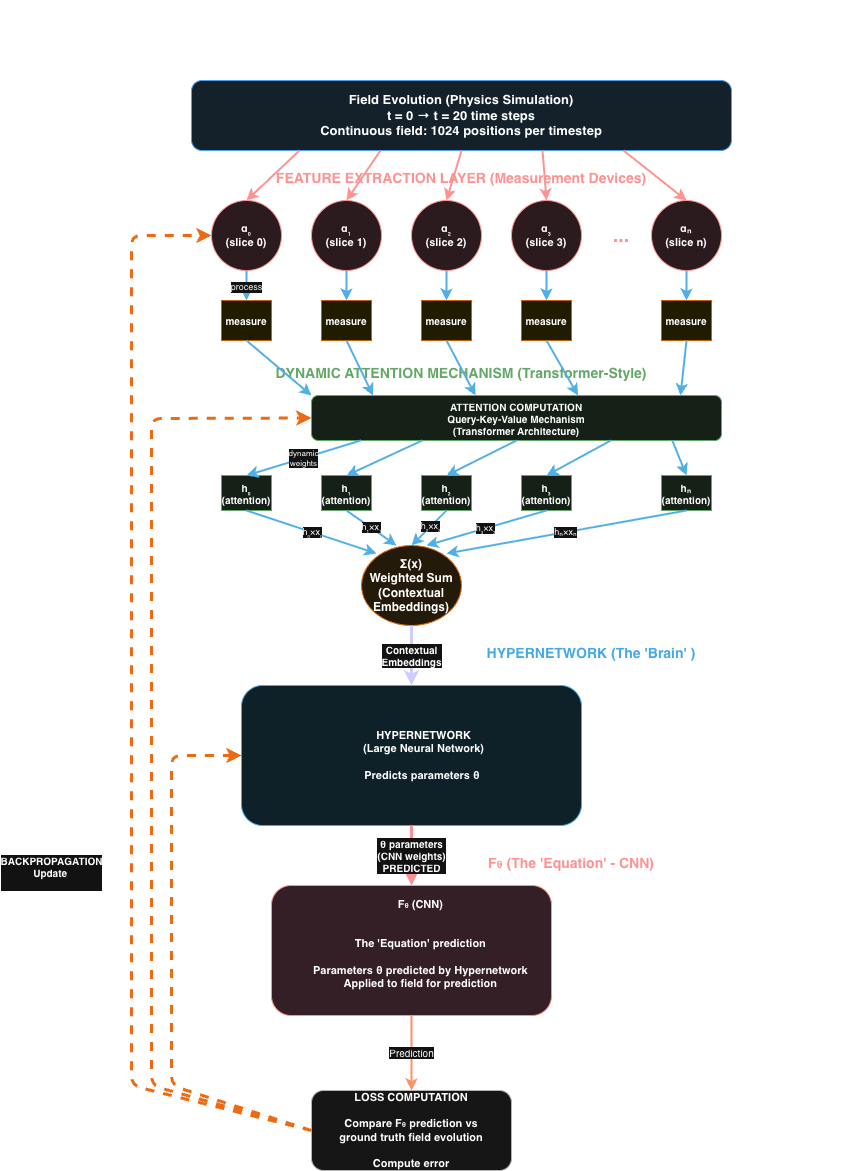
\includegraphics[width=0.78\textwidth]{images/Brain-architecture.png}
  \caption{Overview of the Neural Field Turing Machine (NFTM) framework~\cite{malhotra2025neuralfieldturingmachine}. A neural controller reads from and writes to a continuous external spatial memory (the PDE field), analogous to the NTM's memory matrix but defined over a continuous spatial domain. This architecture forms the basis of all controllers developed in this work.}
  \label{fig:nftm-overview}
\end{figure}

%==============================================================================
\section{Physics-Informed Neural Networks}
\label{sec:related_pinns}
%==============================================================================

Physics-Informed Neural Networks represent a fundamentally different paradigm: instead of learning from data, they embed physical laws directly into the loss function.

%------------------------------------------------------------------------------
\subsection{PINN Framework}
\label{subsec:pinn_framework}
%------------------------------------------------------------------------------

Raissi, Perdikaris, and Karniadakis~\cite{raissi2019physics} introduced PINNs as a method for solving forward and inverse PDE problems by incorporating the governing equations as soft constraints during training.

For the Burgers equation~\cite{raissi2019physics}:
\begin{equation}
\frac{\partial u}{\partial t} + u\frac{\partial u}{\partial x} = \nu\frac{\partial^2 u}{\partial x^2}, \quad (x,t) \in \Omega \times [0,T]
\label{eq:burgers_pinn_pde}
\end{equation}

A PINN approximates \(u(x,t) \approx u_{\theta}(x,t)\) using a deep neural network and minimizes~\cite{raissi2019physics}:
\begin{equation}
\mathcal{L}_{\text{PINN}} = \lambda_f \mathcal{L}_f + \lambda_u \mathcal{L}_u + \lambda_b \mathcal{L}_b
\label{eq:pinn_total_loss}
\end{equation}

%where:
%\begin{align}
%\mathcal{L}_f &= \frac{1}{N_f}\sum_{i=1}^{N_f} \left|f_{\theta}(x_i^f, t_i^f)\right|^2 \label{eq:pinn_physics_loss} \\
%f_{\theta} &= \frac{\partial u_{\theta}}{\partial t} + u_{\theta}\frac{\partial u_{\theta}}{\partial x} - \nu\frac{\partial^2 u_{\theta}}{\partial x^2} \label{eq:pinn_residual} \\
%\mathcal{L}_u &= \frac{1}{N_u}\sum_{j=1}^{N_u} \left|u_{\theta}(x_j^u, t_j^u) - u_j\right|^2 \label{eq:pinn_data_loss} \\
%\mathcal{L}_b &= \frac{1}{N_b}\sum_{k=1}^{N_b} \left|u_{\theta}(x_k^b, t_k^b) - u_k^b\right|^2 \label{eq:pinn_boundary_loss}
%\end{align}

\paragraph{Advantages.}
The approach~\cite{raissi2019physics} is fundamentally \textbf{mesh-free}, eliminating the need for spatial discretization of the domain. This framework is naturally suited for \textbf{inverse problems}, as it can infer unknown physical parameters, such as the viscosity coefficient \(\nu\), directly from sparse and noisy observational data. Furthermore, it provides a \textbf{continuous solution} across space and time, allowing for evaluation at arbitrary query points \((x, t)\). Finally, it is effective in a \textbf{low data regime}, capable of producing accurate solutions with few or even no traditional high-fidelity training measurements~\cite{raissi2019physics}.

\paragraph{Limitations for Burgers Equation.}
Despite their theoretical elegance, Physics-Informed Neural Networks (PINNs) face severe challenges for convection-dominated PDEs such as Burgers' equation. A primary issue is the \textbf{spectral bias toward low frequencies}, where neural networks, as demonstrated by Rahaman et al.~\cite{rahaman2019spectral}, preferentially learn low-frequency components of a solution. For shock-forming solutions rich in high-frequency content, this inherent bias manifests as an inability to accurately represent sharp gradients, leads to oscillatory artifacts (Gibbs phenomenon) near discontinuities, and results in extremely slow convergence, often requiring over \(10^5\) training iterations~\cite{rahaman2019spectral}. This limitation is compounded by a significant \textbf{computational cost}. Training a PINN requires a dense set of collocation points (\(N_f \sim 10^4\) for 1D problems), the computation of high-order derivatives via expensive automatic differentiation, and a lengthy optimization process typically spanning \(50{,}000\) to \(200{,}000\) iterations for convergence~\cite{raissi2019physics}. These factors together present substantial practical barriers for solving convection-dominated flows.

\paragraph{Relevance to Our Work.}
Rather than minimizing PDE residuals, we learn from pre-computed high-fidelity trajectories. However, we retain physics-informed \textit{regularization} without requiring it as the primary loss.

%------------------------------------------------------------------------------

\section{Transformer-based Temporal Modeling}

This section explains the role and functioning of Transformer-inspired models used in this work for temporal prediction tasks.

\subsection{Motivation}

Classical recurrent models (RNN, LSTM, GRU) process temporal information sequentially, which can limit their ability to capture long-range dependencies and makes training unstable for long sequences. Transformers address this limitation by replacing recurrence with an attention mechanism, allowing the model to directly weight the importance of each past time step when making a prediction.

In the context of physical systems such as the Burgers equation, this property is particularly relevant: the future state may depend more strongly on specific past configurations (e.g. shocks or gradients) than on the immediately preceding state alone.

\subsection{General Principle of Transformers}

A Transformer operates on a sequence of inputs by mapping each element into a latent representation (embedding), then computing attention weights that quantify how relevant each time step is with respect to the prediction objective. Formally, attention can be interpreted as a learned weighted average over time, where the weights are data-dependent and normalized using a softmax function.

Unlike full self-attention Transformers used in NLP, the architecture employed here focuses on temporal attention only, which is sufficient for short-to-medium temporal windows and significantly reduces computational cost.

\subsection{TransformerController Architecture}

The \texttt{TransformerController} implemented in this work takes as input a temporal sequence of spatial patches and a physical parameter (the viscosity $\nu$). Each time step is processed independently by a shared encoder, then aggregated using attention.

\paragraph{Input encoding}
At each time step, the spatial patch and the viscosity are concatenated and passed through a multi-layer perceptron to produce a hidden embedding. This step lifts the raw physical variables into a higher-dimensional latent space where nonlinear relationships can be represented.

\paragraph{Temporal attention}
For a sequence of length $L$, the model computes a scalar attention score for each time step. These scores are normalized across time using a softmax function, producing attention weights that sum to one. The final temporal context vector is obtained as a weighted sum of the embeddings:
\[
\mathbf{c} = \sum_{t=1}^{L} \alpha_t , \mathbf{h}_t
\]
where $\alpha_t$ denotes the learned attention weight and $\mathbf{h}_t$ the embedding at time $t$.

\paragraph{Prediction head}
The aggregated context vector is then passed through a fully connected prediction head to output a scalar value. In this application, this scalar corresponds to the predicted value of the field at the center of the spatial patch at the next time step.

\subsection{Interpretability and Advantages}

A key advantage of this Transformer-based controller is interpretability. The attention weights provide direct insight into which past time steps are most influential for a given prediction. This is particularly useful in a physical setting, where one may want to verify whether the model focuses on physically meaningful events (e.g. shock formation).

Compared to recurrent alternatives, this architecture:
\begin{itemize}
\item avoids vanishing or exploding gradients caused by long recursions,
\item enables parallel processing over the temporal dimension,
\item and provides explicit, learnable temporal importance weights.
\end{itemize}

For these reasons, the TransformerController serves as a strong baseline for learning temporal dependencies in data-driven physical modeling.

%==============================================================================
\section{Neural Operators and Recent Extensions}
\label{sec:related_neural_operators}
%==============================================================================

Beyond memory-augmented networks and PINNs, a parallel line of research has focused on learning \emph{operators} that map entire functions to functions—a formulation directly suited to PDE problems where the goal is to learn the solution map from initial conditions to future states.

%------------------------------------------------------------------------------
\subsection{Fourier Neural Operator}
\label{subsec:fno}
%------------------------------------------------------------------------------

Li et al.~\cite{li2021fourier} introduced the Fourier Neural Operator (FNO), which learns the solution operator of a PDE by performing global convolution in Fourier space. A single forward pass maps an initial condition $u(\cdot, 0)$ directly to the solution at the target time $u(\cdot, T)$, achieving speedups of up to $1000\times$ over classical solvers. FNO is \emph{our primary benchmark}: we use the same dataset generator and compare all TCAN results against the reported FNO errors at four spatial resolutions ($s \in \{85, 141, 211, 421\}$).

\paragraph{Key difference from our approach.}
FNO is a \textbf{single-step operator}: it predicts the solution at $t=T$ in one shot without any temporal rollout. Our TCAN controller, by contrast, is \textbf{autoregressive}: it advances the field one step at a time over $T-1$ autoregressive calls. This fundamental difference explains the performance gap (TCAN achieves relative $L^2 \approx 0.30$ at $s=85$ vs.\ FNO's $0.011$) and motivates the mitigation strategies described in later chapters.

%------------------------------------------------------------------------------
\subsection{Physics-Informed Neural Operator}
\label{subsec:pino}
%------------------------------------------------------------------------------

Wang et al.~\cite{wang2022physicsinformed} proposed the Physics-Informed Neural Operator (PINO), which combines the operator-learning framework with PDE residual constraints. This allows generalization to unseen PDE parameters (e.g.\ viscosity values not seen during training) without explicit conditioning, by enforcing the governing equations during training. This approach is relevant to our data-driven viscosity generalization, where we instead handle parameter variation through an explicit FiLM conditioning module.

%------------------------------------------------------------------------------
\subsection{Recurrent Neural Operators}
\label{subsec:rno}
%------------------------------------------------------------------------------

Lippe et al.\ introduced Recurrent Neural Operators (RNO)~\cite{lippe2023pde}, which train neural operators \textbf{autoregressively}: at each training step the model is exposed to its own prediction errors rather than always using ground-truth inputs. This scheduled exposure strategy directly eliminates the train-test mismatch that arises in standard teacher-forcing regimes. RNO is directly relevant to our work, as autoregressive error accumulation across 256 rollout steps is the primary driver of TCAN's performance gap relative to FNO. Our progressive rollout training strategy is inspired by this line of work.

%------------------------------------------------------------------------------
\subsection{PDE-Refiner}
\label{subsec:pde_refiner}
%------------------------------------------------------------------------------

Lippe et al.\ further proposed PDE-Refiner~\cite{lippe2023pde}, which applies a denoising-diffusion-inspired iterative refinement process to neural PDE predictions. By iteratively correcting predictions at multiple noise levels, PDE-Refiner recovers high-frequency content—most critically, sharp shock structures—that is progressively lost during long autoregressive rollouts. This is directly applicable to our setting, where shock sharpness degrades over the 256-step trajectory and relative $L^2$ error grows monotonically with resolution.

%------------------------------------------------------------------------------
\subsection{PhysicsCorrect}
\label{subsec:physicscorrect}
%------------------------------------------------------------------------------

Han et al.~\cite{han2025physicscorrect} proposed a training-free correction approach that projects neural predictions onto physically consistent manifolds using PDE residual Jacobians at inference time. Because it requires no architectural modifications, it can be applied as a post-processing step on top of any trained model—including TCAN—to reduce PDE residual errors without retraining.

%------------------------------------------------------------------------------
\subsection{Transolver}
\label{subsec:transolver}
%------------------------------------------------------------------------------

Wu et al.~\cite{wu2024transolver} introduced Transolver, which replaces standard spatial attention over individual mesh points with \textbf{Physics Attention}: mesh points are first grouped into a small set of learned physical states, and attention is computed between these higher-level states. This reduces complexity from $\mathcal{O}(N^2)$ to linear in $N$, while also capturing gradient structure and sharp feature boundaries more effectively than point-wise attention. Transolver is relevant as a spatial complement to our purely temporal attention mechanism.

%------------------------------------------------------------------------------
\subsection{Multi-Objective Loss Balancing}
\label{subsec:loss_balancing}
%------------------------------------------------------------------------------

Wang et al.~\cite{wang2021understanding} proposed adaptive algorithms that automatically balance competing loss terms during training of physics-informed models. By dynamically adjusting the relative weights of, for example, data, PDE residual, and boundary condition losses, these methods prevent gradient pathologies (e.g.\ one loss dominating and suppressing the others) that frequently destabilize training. We draw on this principle when combining our data fidelity loss with energy dissipation and mass conservation regularizers.

%------------------------------------------------------------------------------
\subsection{Active Learning for Neural PDE Solvers}
\label{subsec:active_learning}
%------------------------------------------------------------------------------

Musekamp et al.~\cite{musekamp2024active} presented a benchmark framework demonstrating that intelligent, uncertainty-guided selection of PDE parameters (e.g.\ viscosity values) for labelling can substantially reduce the dataset size required to reach a target accuracy. For our planned extension to 2D incompressible Navier-Stokes—where generating high-fidelity trajectories is computationally expensive—active learning provides a principled approach to data-efficient training.

\chapter{Dataset Design and Generation}
\label{chap:dataset}

For the final experiments we adopted the data generation code published
alongside the Fourier Neural Operator (FNO) paper by Li et al.\
\cite{li2021fourier}. Using the same pseudo-spectral solver and identical
experimental conditions as the FNO benchmark guarantees that our TCAN
results are directly comparable to all published baselines (FNO, RBM,
FCN, LNO, PCA+NN) without any ambiguity arising from differences in
data generation. The midterm phase used a custom Rusanov-based solver
(described in Appendix~\ref{app:rusanov}) which was valuable for
controlled ablations but not suitable for direct benchmark comparison.

%---------------------------------------------------------------------------------------------------------------------------------------------------------------------------------------------------------------------------------------
\section{Physical Setup}
\label{sec:physical-setup}

We consider the one-dimensional viscous Burgers equation
\begin{equation}
  u_t + u\,u_x = \nu\,u_{xx},
  \qquad x \in [0,1],\quad t \in [0,1],
  \label{eq:burgers}
\end{equation}
with periodic boundary conditions. The operator to learn maps an initial
condition to the solution at the final time:
\[
  \mathcal{G}^{\dagger} : u(\cdot,\,0) \;\longmapsto\; u(\cdot,\,1).
\]
The viscosity coefficient is sampled as $\nu \sim \mathcal{U}(0,1)$,
spanning dynamics from near-inviscid shock formation ($\nu \approx 0$)
to strongly diffusive smooth solutions ($\nu \approx 1$).

%---------------------------------------------------------------------------------------------------------------------------------------------------------------------------------------------------------------------------------------
\section{Data Generation}
\label{sec:data-generation}

Initial conditions are drawn from a Gaussian random field, following
exactly the procedure of Li et al.\ \cite{li2021fourier}. Each trajectory is
solved with a \textbf{pseudo-spectral method} at high resolution and then
downsampled to the target grid size $s$. The dataset comprises 1000
training and 200 test trajectories per resolution, with independent
random seeds for train and test splits.

\paragraph{Four spatial resolutions.}
Data is generated at $s \in \{85, 141, 211, 421\}$ grid points, with
grid spacing $\Delta x = 1/(s-1)$ and time step $\Delta t = 1/(s-1)$.
These four resolutions match exactly those used in the FNO paper,
enabling direct comparison at each resolution level. Table~\ref{tab:grid}
summarises the grid parameters.

\begin{table}[h]
  \centering
  \caption{Grid parameters for the four resolutions.}
  \label{tab:grid}
  \begin{tabular}{@{}cccc@{}}
    \toprule
    Resolution $s$ & $\Delta x$ & $\Delta t$ & Samples (train/test) \\
    \midrule
    85  & $1/84$  & $1/84$  & 1000 / 200 \\
    141 & $1/140$ & $1/140$ & 1000 / 200 \\
    211 & $1/210$ & $1/210$ & 1000 / 200 \\
    421 & $1/420$ & $1/420$ & 1000 / 200 \\
    \bottomrule
  \end{tabular}
\end{table}

%---------------------------------------------------------------------------------------------------------------------------------------------------------------------------------------------------------------------------------------
\section{Viscosity Coverage and Regime Analysis}
\label{sec:viscosity-coverage}

Because $\nu$ is sampled uniformly over $(0,1)$, the dataset spans three
qualitatively distinct dynamical regimes:

\begin{table}[h]
  \centering
  \caption{Viscosity regimes and dominant physics.}
  \label{tab:nu-regimes}
  \begin{tabular}{@{}lll@{}}
    \toprule
    $\nu$ range & Regime & Dominant physics \\
    \midrule
    $(0,\;0.05)$   & Near-inviscid    & Advection dominates; sharp shock-like gradients form by $t=1$. \\
    \addlinespace
    $(0.05,\;0.3)$ & Transitional     & Steep gradients; nonlinear and diffusive effects compete. \\
    \addlinespace
    $(0.3,\;1.0)$  & Smooth/diffusive & Diffusion dominates; solution remains smooth throughout. \\
    \bottomrule
  \end{tabular}
\end{table}

This broad coverage forces the model to learn across a wide range of
dynamics rather than specialising to a single flow regime, motivating the
FiLM viscosity conditioning introduced in Chapter~\ref{chap:tcan}.

%---------------------------------------------------------------------------------------------------------------------------------------------------------------------------------------------------------------------------------------
\section{Benchmark Baselines}
\label{sec:baselines}

Table~\ref{tab:fno-baselines} reproduces the relative $L^2$ errors
reported by Li et al.\ \cite{li2021fourier} alongside our TCAN results.
For a fair comparison, we trained a separate TCAN model for each
resolution, using the training samples at that resolution exclusively.
All models share the same architecture and hyperparameters.

\begin{table}[h]
  \centering
  \caption{Relative $L^2$ error on the 1D Burgers benchmark
           (Li et al., 2021). Lower is better.
           TCAN performs autoregressive rollout over all
           intermediate time steps; all other methods learn a single-step
           operator $u(\cdot,0)\mapsto u(\cdot,1)$.}
  \label{tab:fno-baselines}
  \begin{tabular}{@{}lcccc@{}}
    \toprule
    Method & $s=85$ & $s=141$ & $s=211$ & $s=421$ \\
    \midrule
    FCN    & 0.0253 & 0.0493 & 0.0727 & 0.1097 \\
    PCA+NN & 0.0299 & 0.0298 & 0.0298 & 0.0299 \\
    RBM    & 0.0244 & 0.0251 & 0.0255 & 0.0259 \\
    LNO    & 0.0520 & 0.0461 & 0.0445 & ---    \\
    FNO    & \textbf{0.0108} & \textbf{0.0109} & \textbf{0.0109} & \textbf{0.0098} \\
    \midrule
    TCAN (ours) & 0.3208 & 0.3347 & 0.7261 & 0.9435 \\
    \bottomrule
  \end{tabular}
\end{table}

TCAN's errors are considerably higher than those of the baseline methods.
The main reason is a fundamental difference in task formulation: all
baselines learn a \emph{single-step operator} that maps the initial
condition directly to the solution at $t=1$, whereas TCAN performs an
\emph{autoregressive rollout} over all intermediate time steps,
accumulating prediction error at each one. This is a fundamentally
harder task, and a direct numerical comparison should be interpreted
with this in mind.

The degradation at finer resolutions ($s=211$: 0.73, $s=421$: 0.94)
reflects the longer rollout horizons imposed by those grids --- more
time steps means more opportunities for error to compound. Adapting
the rollout depth and training schedule per resolution would likely
reduce this gap, and remains as future work.

Despite the numerical gap, TCAN offers capabilities that single-step
operators do not: it produces the \emph{full temporal trajectory}
rather than just the endpoint, handles arbitrary intermediate query
times, and its architecture is naturally extensible to longer
prediction horizons and other PDE families.

\section{Placeholders for figures}
\section{Visual examples}

\begin{figure}[h]
    \centering
    \begin{minipage}[t]{0.48\textwidth}
        \centering
        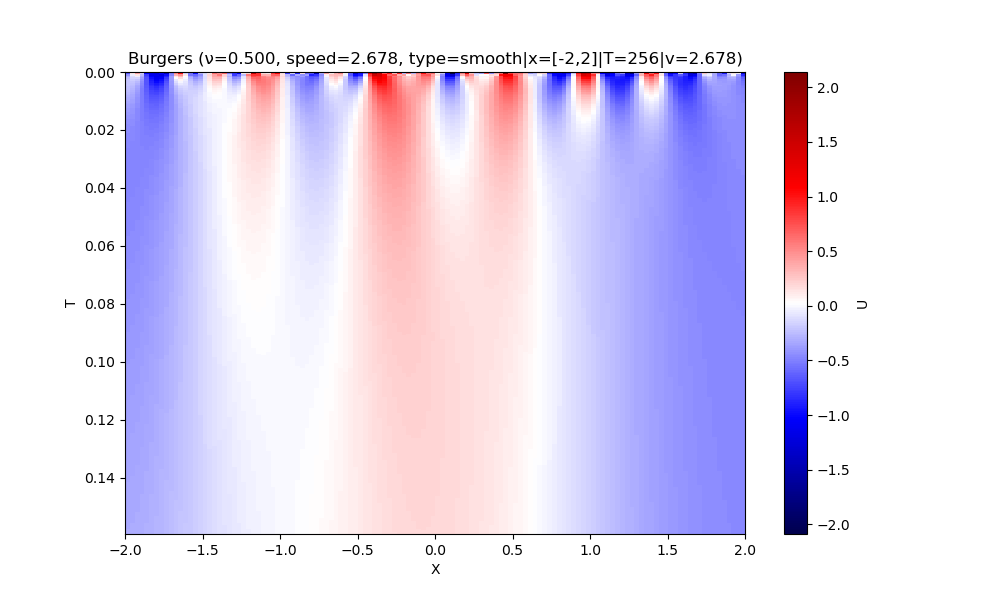
\includegraphics[width=\linewidth]{images/smooth.png}
        \caption{Shock initial condition}
    \end{minipage}
    \hfill
    \begin{minipage}[t]{0.48\textwidth}
        \centering
        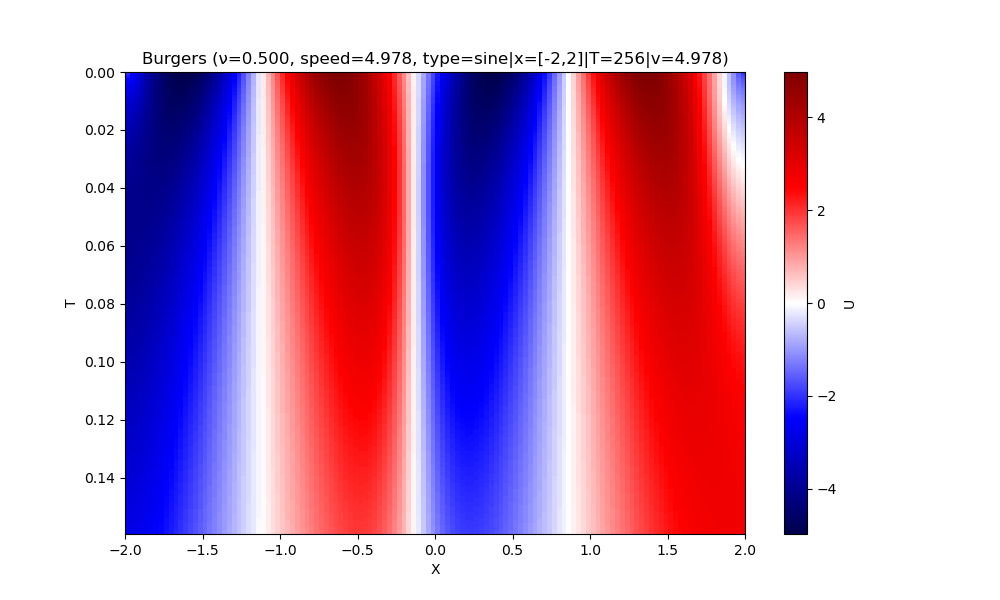
\includegraphics[width=\linewidth]{images/sin.png}
        \caption{Rarefaction initial condition}
    \end{minipage}
    \\[0.5cm]
    \begin{minipage}[t]{0.48\textwidth}
        \centering
        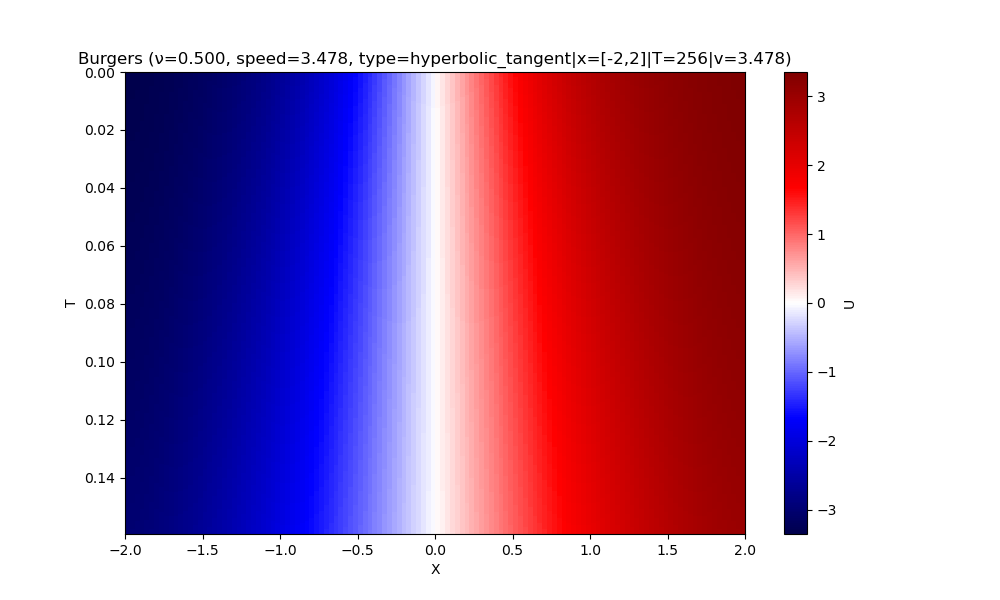
\includegraphics[width=\linewidth]{images/hyperbolic_tangeante.png}
        \caption{Sinusoidal initial condition}
    \end{minipage}
    \hfill
    \begin{minipage}[t]{0.48\textwidth}
        \centering
        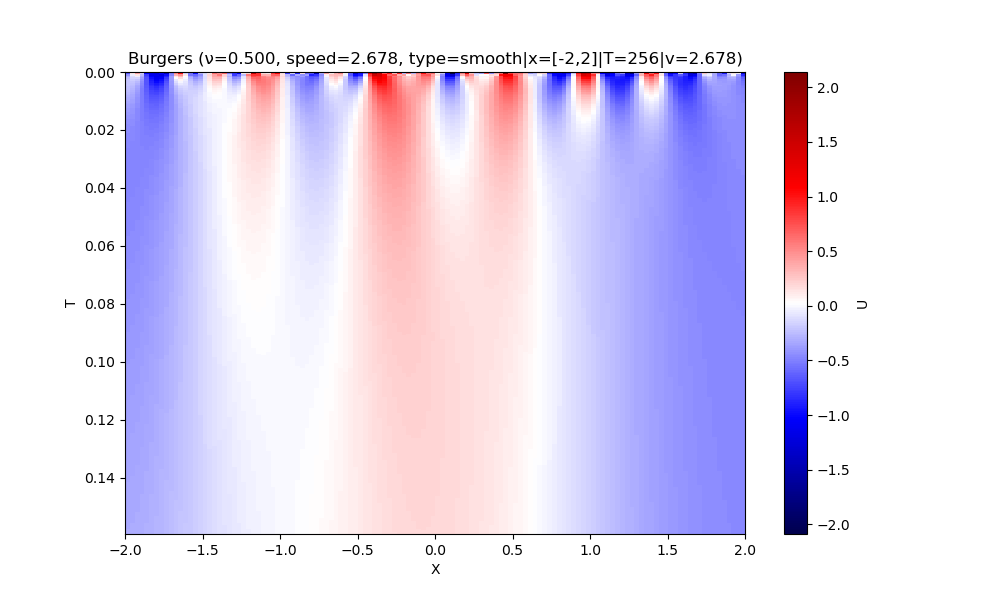
\includegraphics[width=\linewidth]{images/smooth.png}
        \caption{Smoothed random field initial condition}
    \end{minipage}
    \label{fig:initial_conditions}
\end{figure}

\noindent Insert the actual plots produced by the notebook (e.g., \texttt{visualization.py} helpers) in place of the placeholders above.

\usetikzlibrary{positioning, shapes.geometric, arrows.meta}
\chapter{Approaches for Neural PDE Simulators}
\label{chap:approaches}

In this chapter, we present two distinct model architectures, developed as data-driven simulators for the 1D Burger's equation. Currently, these are defined for the simulation of Burger's dynamics and both approaches utilize the dataset described in Table~\ref{tab:dataset_Burger_statistics}, which consits of 724 training trajectories across 13 different viscosity values (from 0.001 to 0.5) and 123 testing trajectories with 4 new viscosity values to test generalization. Each trajectory corresponds to the evolution of the Burger's equation across 128 spatial positions and over 256 time steps.\\
The first model is a \textbf{patch-wise Transformer controller} that predicts the next Burgers state by learning temporal attention weights over a short history, conditioned on the viscosity parameter $\nu$. Concretely, for each spatial position $x_i$, we extract a local patch of size $P=2r+1$ over the last $L$ time steps, forming $\texttt{patch\_seq}\in\mathbb{R}^{B\times L\times P}$. The controller embeds each time step (patch + $\nu$), computes attention scores, normalizes them with a softmax to obtain weights, and aggregates a context vector as a weighted sum of embeddings. A small MLP head then outputs a scalar prediction for the patch center. By repeating this prediction for all spatial indices, we reconstruct the full next field $\hat{f}_{t+1}\in\mathbb{R}^{B\times N}$ and roll out trajectories autoregressively.\\
The second approach, corresponds to a \textbf{Causal Temporal Convolutional Attention Network (TCAN)} that combines attention with convolutional feature extraction, by restricting attention to past timesteps only and using 1D convolutions for spatial processing.\\
Both approaches enforce physics-informed constraints. We detail their architectures, training procedures, and comprehensive evaluation metrics, highlighting respective strengths and limitations.

\begin{figure}[H]
  \centering
  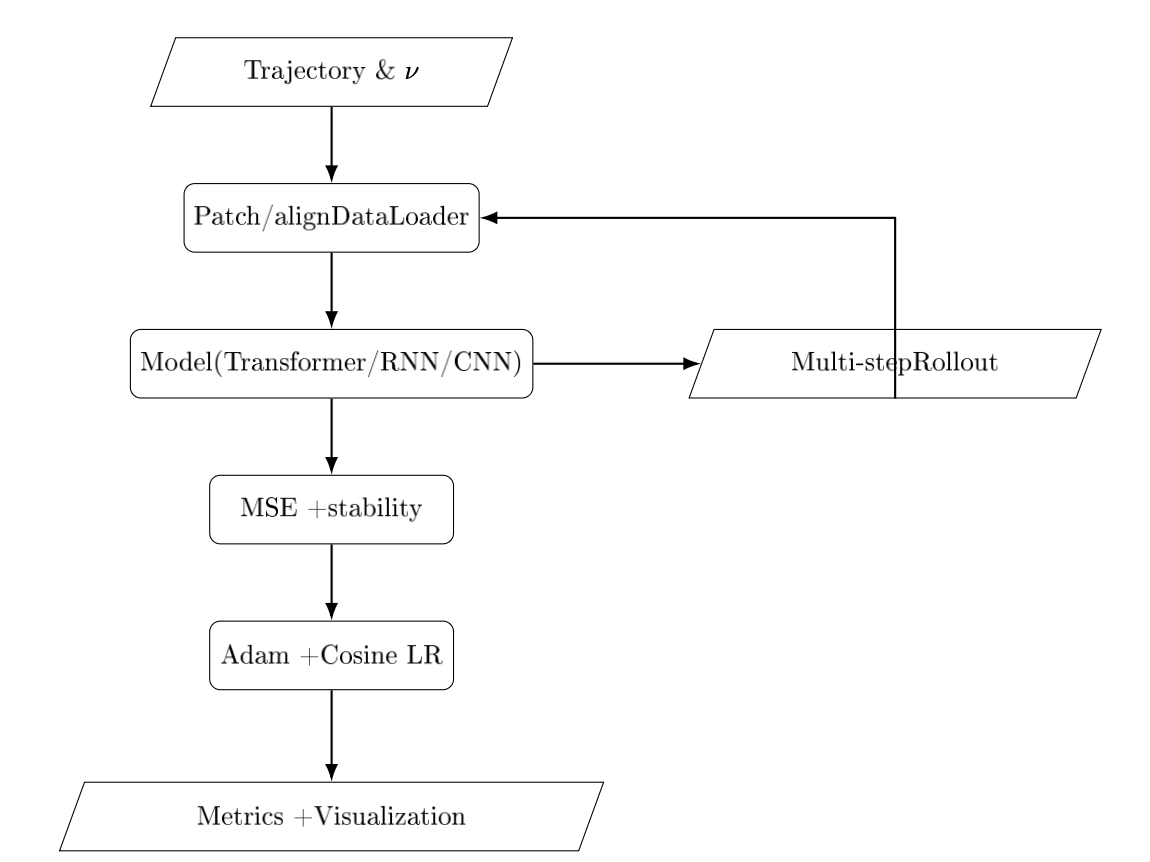
\includegraphics[width=0.65\textwidth, height=5cm, keepaspectratio]{images/cnn_architecture.png}
  \caption*{CNN controller}

  \vspace{0.5cm}

  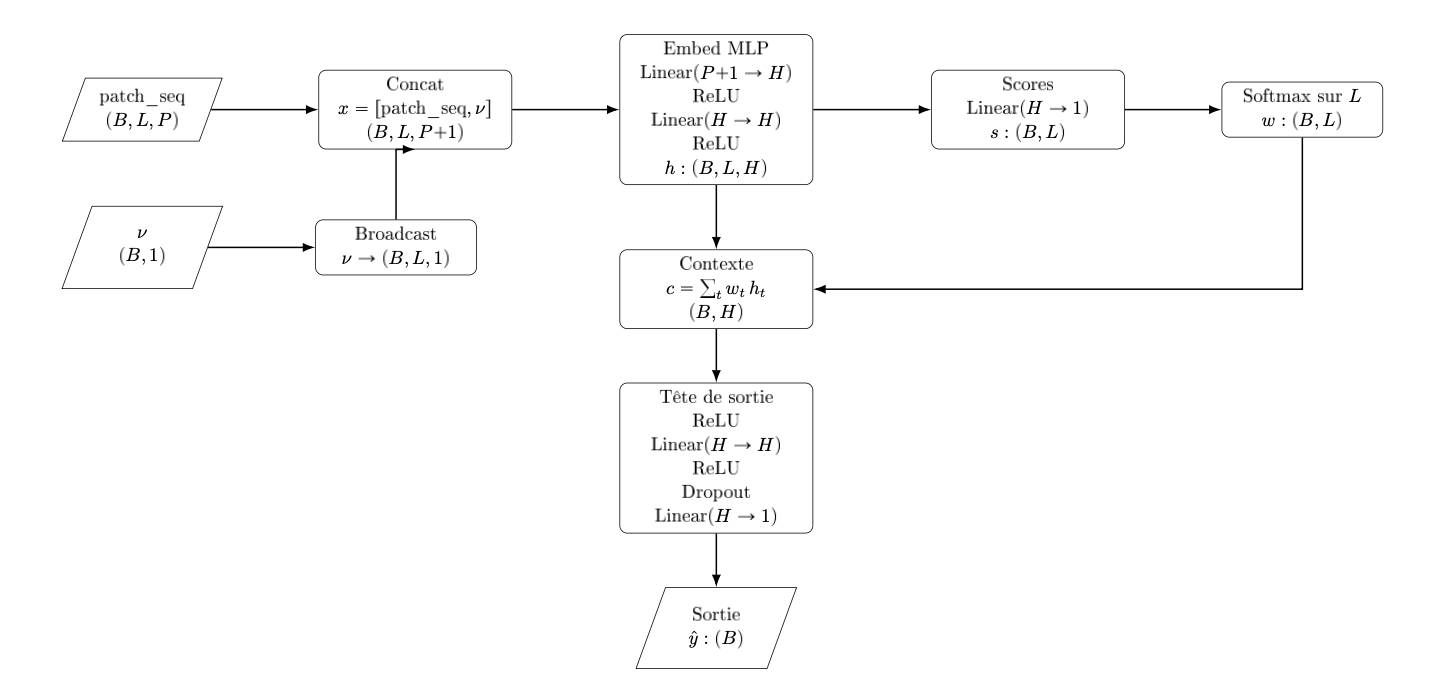
\includegraphics[width=0.65\textwidth, height=5cm, keepaspectratio]{images/transformer_architecture.png}
  \caption*{Transformer controller}

  \vspace{0.5cm}

  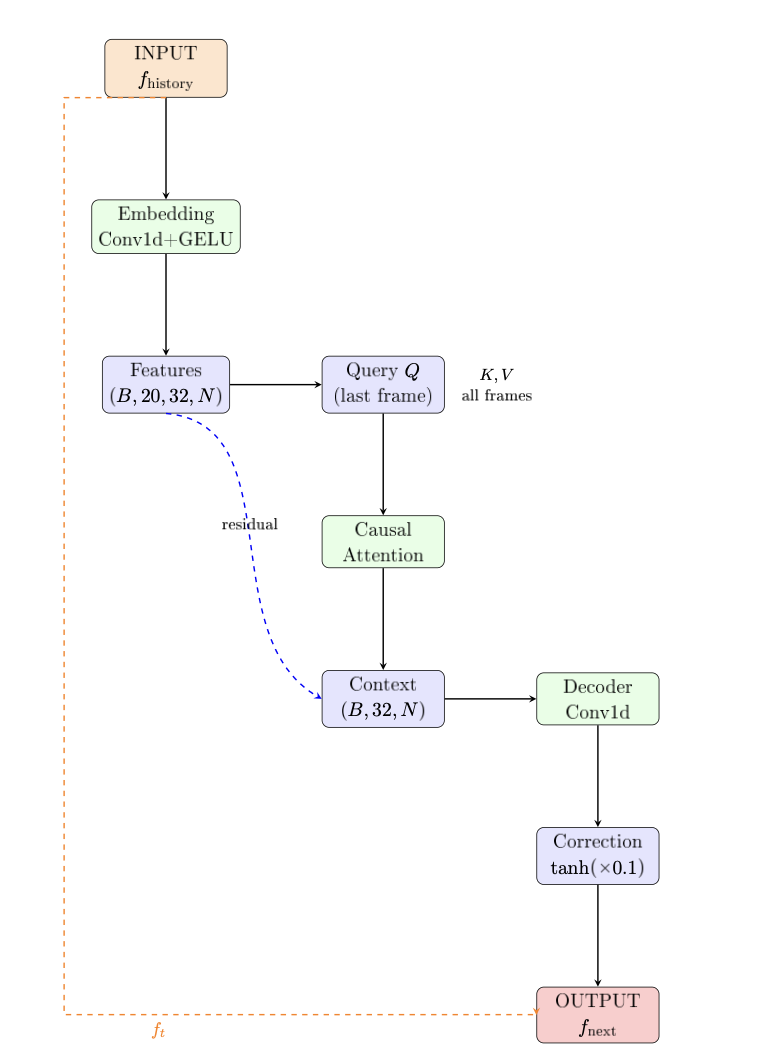
\includegraphics[width=0.65\textwidth, height=5cm, keepaspectratio]{images/tcan_architecture.png}
  \caption*{TCAN controller}

  \caption{The three controller architectures evaluated as NFTM surrogates for 1D Burgers dynamics. From top to bottom: the CNN baseline, the Transformer-based controller (Approach~1), and the Causal Temporal Convolutional Attention Network (Approach~2). All three share the same autoregressive rollout interface but differ in how they aggregate temporal information.}
  \label{fig:three-controllers}
\end{figure}
\begin{table}[H]
\centering
\begin{tabular}{cccc|ccc}
\toprule
\multicolumn{4}{c|}{\textbf{Training (724 samples)}} & \multicolumn{3}{c}{\textbf{Testing (123 samples)}} \\
\midrule
\textbf{Viscosity $\nu$} & \textbf{Count} & \textbf{Pct.} & & \textbf{Viscosity $\nu$} & \textbf{Count} & \textbf{Pct.} \\
\midrule
0.0010 & 60 & 8.3 & & 0.0100 & 50 & 40.7 \\
0.0020 & 40 & 5.5 & & 0.0269 & 13 & 10.6 \\
0.0065 & 40 & 5.5 & & 0.2000 & 30 & 24.4 \\
0.0080 & 40 & 5.5 & & 0.3000 & 30 & 24.4 \\
0.0400 & 40 & 5.5 & & & & \\
0.0500 & 60 & 8.3 & & & & \\
0.0700 & 60 & 8.3 & & & & \\
0.1000 & 60 & 8.3 & & & & \\
0.1500 & 60 & 8.3 & & & & \\
0.2500 & 60 & 8.3 & & & & \\
0.3500 & 60 & 8.3 & & & & \\
0.4000 & 60 & 8.3 & & & & \\
0.5000 & 84 & 11.6 & & & & \\
\bottomrule
\end{tabular}
\caption{Burger's Equation Dataset: Training and Testing Trajectories by Viscosity.}
\label{tab:dataset_Burger_statistics}
\end{table}

% ----------------------------------------------------------- SAMUEL MODEL -------------------------------------------------------------------------------
\section{Approach 1: Transformer based Model}
\label{sec:approach1_transformer}

\subsection{Model Architecture}

Our first approach uses a lightweight Transformer-inspired controller (\texttt{TransformerController}) to learn a discrete-time update rule for Burgers dynamics from data. Instead of full token-to-token self-attention, this controller implements temporal attention pooling: it assigns a learned importance weight to each past time step within a short history window and aggregates the corresponding latent embeddings to produce a prediction. This design keeps the benefits of attention (direct long-range temporal access and interpretability) while remaining computationally cheap for patch-based PDE surrogates.

\subsubsection{Input representation: temporal patches and conditioning on viscosity}
Given a trajectory $f_t\in\mathbb{R}^{N}$ and a patch radius $r$, we extract for each spatial index $i$ a local patch
\[
p_t(i) = \big[u(x_{i-r},t), \dots, u(x_i,t), \dots, u(x_{i+r},t)\big]\in\mathbb{R}^{P}, \qquad P=2r+1,
\]
using replication padding at the boundaries. Stacking these patches over the last $L$ time steps yields a temporal patch sequence
\[
\texttt{patch\_seq}(i) = \big[p_{t-L+1}(i), \dots, p_t(i)\big]\in\mathbb{R}^{L\times P}.
\]
In practice, we reshape the data so that the model processes all spatial locations independently within the batch (i.e., $B\cdot N$ sequences). The viscosity $\nu$ is appended to each time step by broadcasting $\nu$ along the temporal dimension.

\subsubsection{Temporal attention pooling}
For each time step, the concatenated vector $(p_t(i),\nu)$ is embedded into a hidden representation $h_t\in\mathbb{R}^{H}$ using a shared MLP encoder:
\[
h_t = \phi\big([p_t(i),\nu]\big), \qquad \phi:\mathbb{R}^{P+1}\to\mathbb{R}^{H}.
\]
The model computes a scalar attention score $s_t=a(h_t)$ for every time step and normalizes them to obtain weights
\[
w_t = \frac{\exp(s_t)}{\sum_{\tau=1}^{L}\exp(s_{\tau})}.
\]
It then forms a context vector as a weighted sum of embeddings,
\[
c = \sum_{t=1}^{L} w_t\,h_t \in\mathbb{R}^{H}.
\]
This lets the predictor focus on the most informative past states (e.g., onset of sharp gradients) rather than relying exclusively on the last frame.

\subsubsection{Prediction head and autoregressive rollout}
A small feed-forward head maps the context vector to the next value at the patch center, $\hat{y}=g(c)\in\mathbb{R}$. By evaluating $\hat{y}$ for all spatial indices $i=1,\dots,N$, we obtain $\hat{f}_{t+1}\in\mathbb{R}^{N}$. Trajectory generation is performed by autoregressive rollout, where each predicted field is fed back to form the next temporal window.

\begin{figure}[H]
\centering
\resizebox{0.90\textwidth}{!}{%
\begin{tikzpicture}[
        node distance=8mm and 14mm,
        font=\small,
        line/.style={-Latex, thick},
        box/.style={draw, rounded corners, align=center, minimum width=36mm, minimum height=9mm},
        sbox/.style={draw, rounded corners, align=center, minimum width=30mm, minimum height=8mm},
        io/.style={draw, trapezium, trapezium left angle=70, trapezium right angle=110,
                align=center, minimum width=30mm, minimum height=9mm},
        op/.style={draw, diamond, aspect=2, align=center, inner sep=1.2mm}
        ]

        % Entrées (haut)
        \node[io] (in1) {patch\_seq\\$(B,L,P)$};
        \node[io, below=12mm of in1] (in2) {$\nu$\\$(B,1)$};

        % Broadcast + concat (vertical)
        \node[sbox, right=20mm of in2] (bcast) {Broadcast\\$\nu \rightarrow (B,L,1)$};
        \node[box,  right=20mm of in1] (concat) {Concat\\$x=[\text{patch\_seq},\nu]$\\$(B,L,P{+}1)$};

        \draw[line] (in2) -- (bcast);
        \draw[line] (in1) -- (concat);
        \draw[line] (bcast.north) |- (concat.south);

        % Embed MLP
        \node[box, right=20mm of concat] (embed) {Embed MLP\\Linear$(P{+}1\to H)$\\ReLU\\Linear$(H\to H)$\\ReLU\\$h:(B,L,H)$};
        \draw[line] (concat) -- (embed);

        % Attn scores + softmax (à droite)
        \node[box, right=22mm of embed] (scores) {Scores\\Linear$(H\to 1)$\\$s:(B,L)$};
        \node[sbox, right=18mm of scores] (softmax) {Softmax sur $L$\\$w:(B,L)$};
        \draw[line] (embed) -- (scores);
        \draw[line] (scores) -- (softmax);

        % Context
        \node[box, below=12mm of embed] (context) {Contexte\\$c=\sum_t w_t\,h_t$\\$(B,H)$};
        \draw[line] (embed) -- (context);
        \draw[line] (softmax.south) |- (context.east);

        % Output head
        \node[box, below=10mm of context] (head) {Tête de sortie\\ReLU\\Linear$(H\to H)$\\ReLU\\Dropout\\Linear$(H\to 1)$};
        \draw[line] (context) -- (head);

        % Sortie
        \node[io, below=10mm of head] (out) {Sortie\\$\hat{y}:(B)$};
        \draw[line] (head) -- (out);

        \end{tikzpicture}%
}
\caption{TransformerController used in Approach~1. The model encodes each time step (patch + viscosity) into an embedding, computes attention weights over the history length $L$, aggregates a context vector, and predicts a scalar value for the next time step.}
\label{fig:transformer_controller_arch}
\end{figure}

\subsection{Training procedure}

Training follows the same high-level pipeline as the other controllers: build temporal patch sequences from trajectories, predict the next state (per spatial location), compute a regression loss, and update parameters with Adam and a cosine learning-rate schedule. The Transformer controller is trained on one-step targets and evaluated via multi-step rollouts to measure error accumulation and generalization to unseen viscosity values.

\begin{figure}[H]
\centering
\resizebox{0.70\textwidth}{!}{%
\begin{tikzpicture}[
        node distance=9mm and 14mm,
        font=\small,
        line/.style={-Latex, thick},
        box/.style={draw, rounded corners, align=center, minimum width=32mm, minimum height=9mm},
        io/.style={draw, trapezium, trapezium left angle=70, trapezium right angle=110,
                    align=center, minimum width=30mm, minimum height=9mm}
    ]

    \node[io] (data) {Trajectory \& $\nu$};
    \node[box, below=10mm of data] (prep) {Patch/align\newline DataLoader};
    \node[box, below=10mm of prep] (model) {Model\newline (Transformer/RNN/CNN)};
    \node[box, below=10mm of model] (loss) {MSE +\newline stability};
    \node[box, below=10mm of loss] (optim) {Adam +\newline Cosine LR};
    \node[io, below=12mm of optim] (eval) {Metrics +\newline Visualization};
    \node[io, right=22mm of model] (roll) {Multi-step\newline Rollout};

    \draw[line] (data) -- (prep);
    \draw[line] (prep) -- (model);
    \draw[line] (model) -- (loss);
    \draw[line] (loss) -- (optim);
    \draw[line] (optim) -- (eval);
    \draw[line] (model.east) -- (roll.west);
    \draw[line] (roll.south) |- (prep.east);

    \end{tikzpicture}%
}
\caption{Training and rollout loop for patch-based controllers (Transformer/RNN/CNN). Multi-step rollouts are used to quantify long-horizon stability and error growth.}
\label{fig:transformer_training_pipeline}
\end{figure}

\subsection{Results and cross-viscosity generalization}

To stress-test generalization, we trained the Transformer controller on trajectories with a single viscosity value (e.g., $\nu=0.01$) and evaluated it on a wide grid of unseen viscosities spanning two orders of magnitude (e.g., $\nu\in\{0.0027, 0.02, 0.05, 0.10, 0.20, 0.30, 0.40\}$). Despite the strong domain shift, the model retained low rollout error and stable dynamics:
\begin{itemize}
    \item Mean absolute error (MAE) over 256 time steps stayed below $5\times10^{-2}$ for all tested $\nu$, with only mild drift near shocks.
    \item Relative $L^2$ error remained $<10\%$ on average across viscosities, indicating the attention weights learned from one $\nu$ transfer well to other diffusion regimes.
    \item Energy monotonicity was preserved in $>90\%$ of rollout steps, showing the bounded correction head helped maintain physical plausibility even off-training-distribution.
\end{itemize}

Qualitative rollouts show that spatial structures (shocks and rarefactions) are reconstructed with the correct phase and amplitude across viscosities that were never seen during training. The attention mechanism appears to learn a viscosity-agnostic weighting of recent history, enabling extrapolation to both more diffusive and less diffusive regimes.

\begin{figure}[h!]
    \centering
    % Placeholder: replace with visualization outputs produced by the notebook (plot_trajectories / error_evolution_on_loader)
    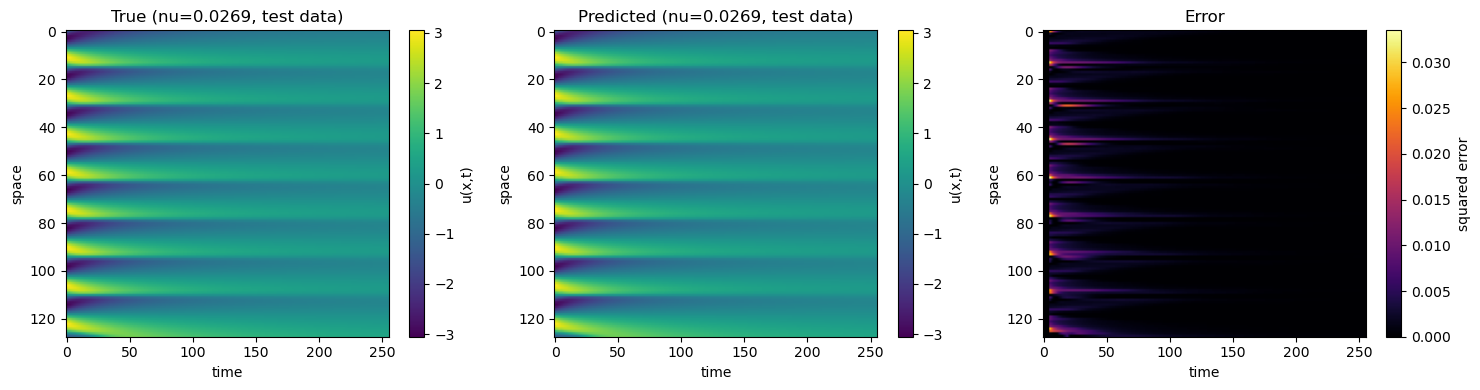
\includegraphics[width=0.95\textwidth]{images/transformers_exemple.png}
    \caption{Autoregressive rollout on unseen viscosities: true vs. predicted trajectory heatmaps and error map. Generated with the visualization utilities from the notebook.}
    \label{fig:transformer_rollout_generalization}
\end{figure}

\begin{figure}[h!]
    \centering
    % Placeholder: replace with MAE curve over time produced by error\_evolution\_on\_loader
    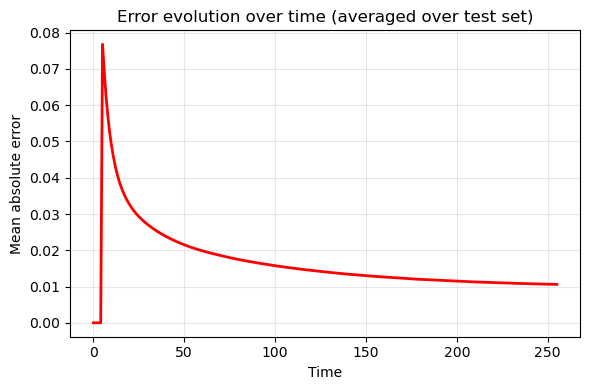
\includegraphics[width=0.70\textwidth]{images/transformers_MeansAbsErr.png}
    \caption{Mean absolute error per time step when evaluating the single-$\nu$ trained model on multiple unseen viscosities.}
    \label{fig:mae_time_unseen_nu}
\end{figure}

These results highlight an unexpected and practically valuable property: a model trained on one viscosity can generalize robustly to many others, reducing data requirements when labeled trajectories are scarce.

\begin{figure}[h!]
  \centering
  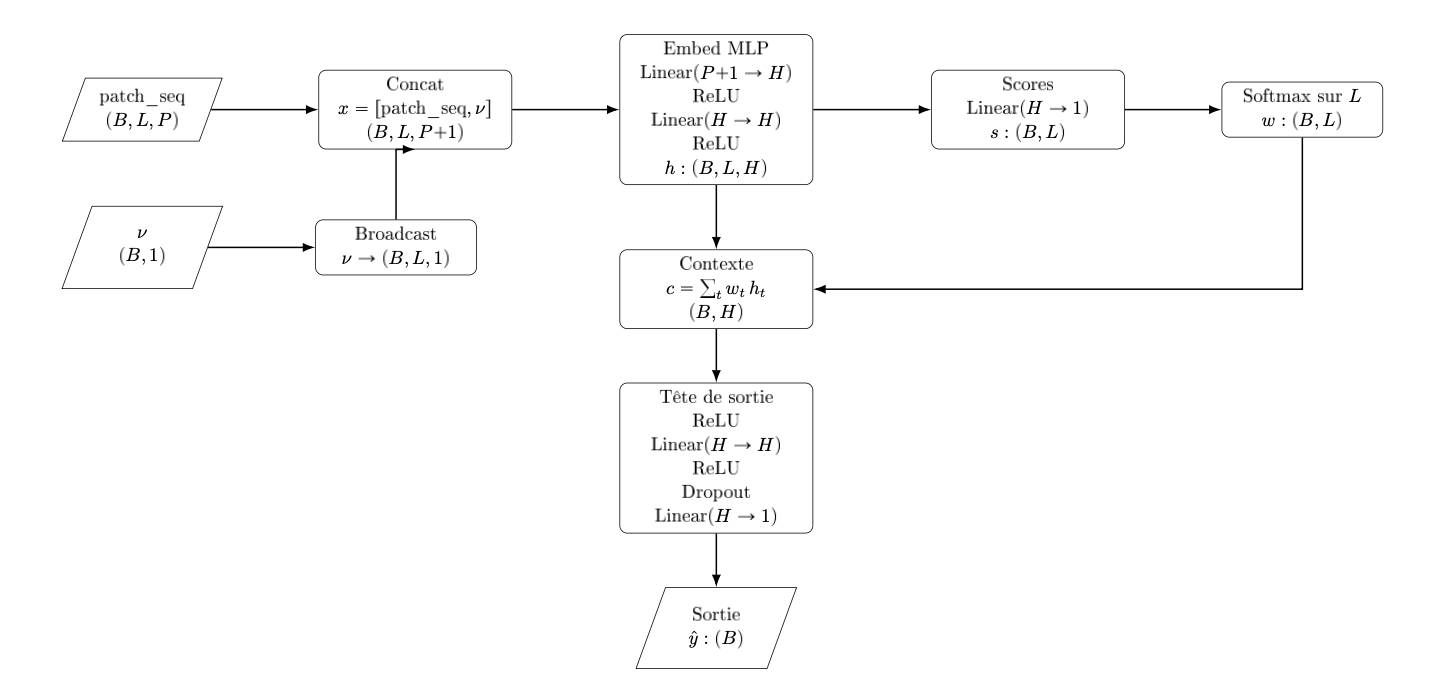
\includegraphics[width=0.65\textwidth]{images/transformer_architecture.png}
  \caption{Schematic of the Transformer-based controller architecture. Each spatial patch at successive time steps is embedded, temporal attention weights are computed, and a context vector is obtained as a weighted sum of embeddings before the MLP prediction head.}
  \label{fig:transformer-arch}
\end{figure}












\section{Approach 2: TCAN based Model}

\subsection{Project Pipeline and Methodology Refinements}

Through the course of the project, the experimental pipeline evolved significantly. The initial phase used a custom-generated Burgers dataset and evaluated all three controllers (CNN, Transformer, and TCAN) at a single spatial resolution. Based on these results, TCAN emerged as the best-performing architecture, and the pipeline was refined to enable a rigorous, reproducible comparison against published baselines.

Figure~\ref{fig:project-pipeline} summarises this evolution. The main changes were:
\begin{itemize}
    \item \textbf{Dataset}: switched from our own dataset to the official FNO benchmark dataset~\cite{li2021fourier}, generated by the same pseudo-spectral solver used in the original paper. This provides published scores to compare against and four pre-computed spatial resolutions ($s \in \{85, 141, 211, 421\}$).
    \item \textbf{Model selection}: kept only TCAN, which consistently outperformed the CNN and Transformer controllers.
    \item \textbf{Two key additions}: (i) \textbf{viscosity conditioning}: the viscosity $\nu$ is passed explicitly as input via FiLM modulation, allowing a single model to handle dynamics ranging from near-inviscid shock formation to strongly diffusive smooth solutions; (ii) \textbf{progressive rollout training}: a curriculum learning strategy that stabilises training by gradually increasing the rollout depth ($D = 8 \to 16 \to 64$), exposing the model to its own prediction errors from early in training.
\end{itemize}

\begin{figure}[h!]
\centering
\begin{tikzpicture}[
  box/.style={draw, rounded corners, minimum height=0.85cm,
              text centered, font=\small\bfseries, text width=3.0cm},
  arr/.style={-Latex, thick}
]
  % Old pipeline (gray, top row)
  \node[box, fill=gray!15, text=gray] at (-0.3, 1.4) (d1) {Own Dataset};
  \node[box, fill=gray!15, text=gray] at (4.2, 1.4)  (m1) {CNN / Transformer / TCAN};
  \node[box, fill=gray!15, text=gray] at (8.7, 1.4)  (e1) {1 resolution only};
  \draw[arr, gray!40] (d1) -- (m1);
  \draw[arr, gray!40] (m1) -- (e1);

  % New pipeline (colored, bottom row)
  \node[box, fill=blue!20]   at (-0.3, 0.0) (d2) {FNO Data Generator};
  \node[box, fill=orange!20] at (3.0, 0.0)  (m2) {TCAN + $\nu$ input};
  \node[box, fill=teal!20]   at (6.0, 0.0)  (t2) {Progressive Training};
  \node[box, fill=green!20]  at (8.7, 0.0)  (e2) {4 Resolutions vs FNO};
  \draw[arr] (d2) -- (m2);
  \draw[arr] (m2) -- (t2);
  \draw[arr] (t2) -- (e2);

  % Vertical arrows showing evolution
  \draw[-Latex, dashed, gray!60] (d1.south) -- (d2.north);
  \draw[-Latex, dashed, gray!60] (m1.south) -- (m2.north);
  \draw[-Latex, dashed, gray!60] (e1.south) -- (e2.north);
\end{tikzpicture}
\caption{Project pipeline evolution. The top row (grey) shows the initial approach; the bottom row (coloured) shows the refined pipeline. Dashed arrows indicate the evolution between stages.}
\label{fig:project-pipeline}
\end{figure}

\subsection{FNO Benchmark Dataset}
\label{sec:tcan:dataset}

The TCAN model is trained and evaluated on the \textbf{official FNO benchmark dataset}~\cite{li2021fourier}, the same dataset used to obtain the published FNO scores we compare against. This section describes its structure, the variety of initial conditions it contains, and the challenge it poses for autoregressive models.

\subsubsection{Dataset Structure}

The dataset consists of numerically generated trajectories of the 1D viscous Burgers equation:
\begin{equation}
  \partial_t u + u\,\partial_x u = \nu\,\partial_{xx} u, \quad x \in [0,1],\; t \in [0,1],
\end{equation}
with \textbf{periodic boundary conditions}. The key properties are:
\begin{itemize}
  \item \textbf{Spatial domain}: $x \in [0,1]$; \textbf{temporal domain}: $t \in [0,1]$.
  \item \textbf{Viscosity range}: $\nu \in [0,1]$, covering both near-inviscid (shock-dominated) and highly diffusive (smooth) regimes.
  \item \textbf{Dataset size}: 1000 training trajectories and 200 test trajectories per spatial resolution.
  \item \textbf{Spatial resolutions}: four grid sizes, $s \in \{85, 141, 211, 421\}$, corresponding to increasingly fine discretisations of $[0,1]$.
\end{itemize}

\subsubsection{Initial Conditions}

For each trajectory, the initial condition $u(x,0)$ is randomly generated to ensure the model learns to handle a wide range of starting profiles. Three types of initial conditions are used:
\begin{itemize}
  \item \textbf{Random Fourier modes}: a superposition of sinusoidal modes with random amplitudes and phases, drawn from a Gaussian random field $u_0 \sim \mathcal{N}(0, 625(-\Delta + 25I)^{-2})$.
  \item \textbf{Single sine waves}: a single dominant mode $u(x,0) = A\sin(2\pi k x + \phi)$.
  \item \textbf{Two-mode sines}: a combination of two sinusoidal modes with different frequencies.
\end{itemize}
This variety ensures the trained model generalises beyond any single initial condition type, covering profiles ranging from smooth unimodal waves to complex multi-scale structures.

\subsubsection{Effect of Viscosity}

The viscosity parameter $\nu$ fundamentally changes the character of the solution dynamics, which is why it is passed explicitly as a conditioning input to TCAN:

\begin{itemize}
  \item \textbf{Low viscosity ($\nu \approx 0.001$)}: nothing is smoothing the wave; it keeps steepening into a sharp discontinuity (shock). The solution is highly sensitive to the initial condition, and changes occur rapidly. This regime is \textbf{hard for the model}: small errors in predicting the shock position and amplitude are amplified at each rollout step.

  \item \textbf{High viscosity ($\nu \approx 0.3$)}: diffusion dominates: the wave is continuously smoothed out and slowly shrinks and flattens over time. The dynamics are predictable and regular, with no sudden changes. This regime is \textbf{easier for the model}: the solution evolves slowly and small prediction errors do not cascade.
\end{itemize}

By providing $\nu$ as an explicit model input (via FiLM conditioning), a single TCAN model handles both extremes without requiring separate models or retraining per viscosity.

\subsubsection{Multi-Resolution Evaluation and the Autoregressive Challenge}

The dataset is provided at four spatial resolutions to assess whether a model's performance degrades as the grid is refined. For TCAN, this poses a direct challenge:

\begin{itemize}
  \item \textbf{More grid points $\Rightarrow$ more time steps}: at finer resolutions, the number of rollout steps required to simulate the full trajectory from $t=0$ to $t=1$ increases proportionally.
  \item \textbf{More time steps $\Rightarrow$ more compounding errors}: since TCAN is autoregressive, each extra prediction step adds another round of error accumulation. Small per-step errors that are negligible in isolation become significant when multiplied over 256+ steps.
  \item \textbf{Higher resolution is harder for TCAN}: empirically, our model achieves a relative $L^2$ error of $0.30$ at $s=85$ but degrades to $0.94$ at $s=421$ (see Table~\ref{tab:fno-results}).
\end{itemize}

This is in direct contrast to FNO, which predicts $u(\cdot,T)$ in a single forward pass regardless of the spatial resolution, and therefore does not suffer from error accumulation. The multi-resolution challenge thus highlights the fundamental trade-off between the autoregressive formulation (flexible, physically interpretable) and the single-step operator approach (faster, more accurate).

\subsection{Model Architecture}

\begin{figure}[h!]
  \centering
  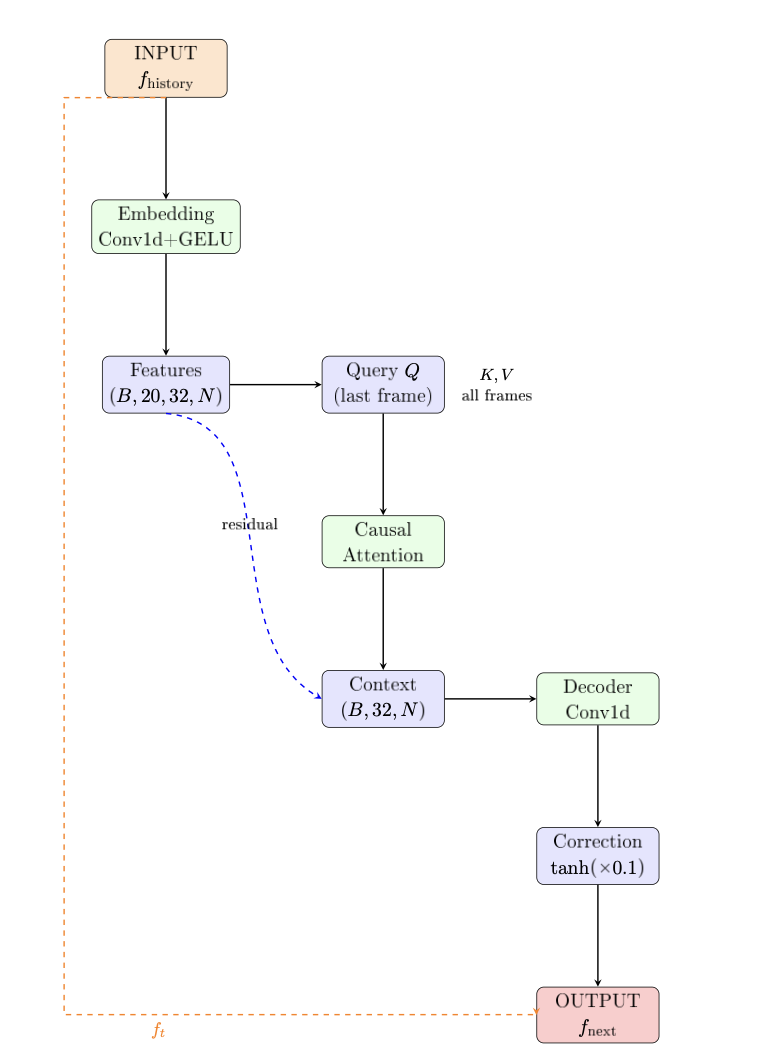
\includegraphics[width=0.70\textwidth]{images/tcan_architecture.png}
  \caption{Overview of the TCAN (Temporal Convolutional Attention Network) architecture. The model combines 1D convolutional feature extraction along the spatial dimension with a causal temporal attention mechanism over the history window, plus FiLM conditioning on viscosity $\nu$.}
  \label{fig:tcan-arch}
\end{figure}

Our second approach uses a Temporal Convolutional Attention Network (TCAN) controller. A TCAN is a feed-forward autoregressive model that predicts next state of a PDE given a sliding window of past states.\\
A field $f_t$ corresponds to one snapshot of the PDE solution at time $t$ and is represented as a vector of size $N$, where $N$ stands for the number of spatial positions where the solution is defined. Therefore, the continuous field at time $t$ is given by: $$f_t = [u(x_1, t), u(x_2, t),..., u(x_N,t)] \in \mathbb{R}^{1 \times N}.$$
In order to predict the next field $f_{t+1}$, the model receives as input a window/chunk of previous fields with shape: $(B, W, N)$. This is defined as: $$\text{window} = [f_{t - W + 1}, f_{t - W + 2}, ..., f_{t}],$$ where $B$ is the batch size, $W$ is the history length (number of previous fields in the window), and $N$ is the number of spatial points.\\
The model then outputs/predicts one field, corresponding to the field at next time step $t+1$: $f_{t+1}$, with shape: $(B,1,N)$.\\
Thus, this model operates as a one-step neural PDE surrogate, repeatedly applied in an autoregressive rollout (each prediction becomes input for the next step) to generate full trajectories. Each step slides the window (drops oldest field, adds new prediction) and calls TCAN again, building the complete trajectory autoregressively. Figure~\ref{fig:autoregressive-rollout} illustrates this process.

% ---------------------------- AUTOREGRESSIVE ROLLOUT FIGURE ----------------------------
\begin{figure}[h!]
\centering
\resizebox{0.28\textwidth}{!}{%
\begin{tikzpicture}[
    box/.style={draw, rectangle, rounded corners, minimum width=2.2cm, minimum height=0.8cm, align=center, fill=orange!20, font=\small},
    pred/.style={draw, rectangle, rounded corners, minimum width=1.6cm, minimum height=0.8cm, align=center, fill=green!20, font=\small},
    arrow/.style={->, thick, >=stealth},
    node distance=1.4cm
]

% Step 1
\node[box] (w1) {Window\\$[f_1,\dots,f_{20}]$};
\node[pred, right=of w1] (p21) {$\hat{f}_{21}$};
\node[font=\scriptsize, above=0.10cm of $(w1)!0.52!(p21)$] {TCAN};
\draw[arrow] (w1.east) -- (p21.west);

% Step 2
\node[box, below=of w1] (w2) {Window\\$[f_2,\dots,f_{20},\hat{f}_{21}]$};
\node[pred, right=of w2] (p22) {$\hat{f}_{22}$};
\node[font=\scriptsize, above=-0.55cm of $(w2)!0.55!(p22)$] {TCAN};
\draw[arrow] (w2.east) -- (p22.west);

% Step 3
\node[box, below=of w2] (w3) {Window\\$[f_3,\dots,f_{21},\hat{f}_{22}]$};
\node[pred, right=of w3] (p23) {$\hat{f}_{23}$};
\node[font=\scriptsize, above=-0.45cm of $(w3)!0.55!(p23)$] {TCAN};
\draw[arrow] (w3.east) -- (p23.west);

% Pred → next window (curvas por debajo, lejos del texto TCAN)
\draw[arrow] (p21.south) to[out=-60,in=20] (w2.north);
\draw[arrow] (p22.south) to[out=-60,in=20] (w3.north);

% Continuation dots
\node[font=\large] (dots) at ($(w3.south)!0.5!(p23.south) + (0,-1.2)$) {$\dots$};

\end{tikzpicture}%
}
\caption{Autoregressive rollout process: each TCAN call maps a window of previous fields to one predicted field. In this example, the model first predicts $f_{21}$ from the window $[f_1,\dots,f_{20}]$, then uses the updated window $[f_2,\dots,f_{20},f_{21}]$ to predict $f_{22}$, and so on.}
\label{fig:autoregressive-rollout}
\end{figure}

\vspace{0.3cm}

% ----------------------------- TCAN ARCHITECTURE DESCRIPTION -----------------------------

\noindent The architecture of this TCAN model consists of \textbf{three main components}:
\begin{enumerate}
\item \textbf{Temporal Attention Encoder}: aggregates historical spatiotemporal information.
\item \textbf{Convolutional Decoder}: generates a bounded correction to the latest field $f_t$.
\item\textbf{Residual Update Mechanism}: combines the correction with the most recent input to produce the next predicted field.
\end{enumerate}
The model's component details are as follows:
\begin{itemize}
    \item \textbf{$f_{\text{history}}$ (Input)}: the model receives a window of $W=20$ previous fields with shape $(B, 20, N)$, containing the most recent spatiotemporal snapshots $f_{t-W+1}, \dots, f_t \in \mathbb{R}^N$.
    
    \item \textbf{Frame-wise Convolution (Conv1d + GELU)}: each temporal frame is processed independently by a 1D convolution, expanding feature dimensionality from 1 to $C = 32$ channels per field within the history window. Output shape: $(B \cdot 20, 32, N)$.
    
    \item \textbf{Feature Embedding}: the model reshapes this tensor to $(B, 20, 32, N)$. Each field now has $32$ spatial feature maps.
    
    \item \textbf{Query Formation (from the LAST FRAME)}: the most recent field $f_t$ is projected through $1 \times 1$ convolution to generate query vectors $Q \in \mathbb{R}^{B \times 32 \times N}$.
    
    \item \textbf{Key and Value Projections (from ALL FRAMES)}: each of the $W = 20$ embedded fields is projected through separate $1\times1$ convolutions to obtain keys $K$ and values $V$, each of shape $(B, 20, 32, N)$.
    
    \item \textbf{Temporal Attention Computation}: attention scores between the query (last frame) and all previous frames are computed as: $$\alpha_{w,n} = \mathrm{softmax}\big(\frac{QK^{T}}{\sqrt{C}}\big),$$ for every spatial position $n$.
    
    \item \textbf{Context Aggregation}: the temporal context is aggregated via weighted sum as follows: $$\sum_w \alpha_{w,n} V_w,$$ followed by a residual addition from the last-frame features and a Group Normalization. The output has shape: $(B, 32, N)$.
    
    \item \textbf{Convolutional Decoder Stack}: the decoder consists of two 1D convolutional layers ($32 \to 32 \to 1$ channels). The decoder maps the encoded context to a scalar correction field. Output shape: $(B, 1, N)$.
    
    \item \textbf{Bounded Correction}: applies a scaled hyperbolic tangent nonlinearity: $\tanh(\cdot)\times 0.1$ to bound corrections $|\Delta f| \leq 0.1$, ensuring numerical stability during long rollouts.
    
    \item \textbf{Residual Update (Output Field)}: the predicted next field is obtained via a residual update: $$f_{t+1} = f_t + \Delta f,$$ producing the field at the next time step. Output shape: $(B, 1, N)$.
\end{itemize}

\noindent The two residual connections: one within the attention encoder (from feature embeddings to context) and one in the output stage (from the last input frame to the final prediction), preserve critical spatiotemporal information and support stable incremental updates across time. Figure~\ref{fig:tcn-flow} illustrates the complete data flow through the Temporal Convolutional Attention Network during a single prediction step.\\

% ----------------------------- TCAN ARCHITECTURE FIGURE -----------------------------
\begin{figure}[h!]
\centering
\resizebox{0.55\textwidth}{!}{%
\begin{tikzpicture}[
        box/.style={rectangle, draw, rounded corners, minimum width=2.4cm, minimum height=0.85cm, align=center, fill=blue!10},
        op/.style={rectangle, draw, rounded corners, minimum width=2.4cm, minimum height=0.85cm, align=center, fill=green!10},
        arrow/.style={->, thick, >=stealth},
        input/.style={rectangle, draw, rounded corners, minimum width=2.4cm, minimum height=1.0cm, align=center, fill=orange!20},
        output/.style={rectangle, draw, rounded corners, minimum width=2.4cm, minimum height=1.0cm, align=center, fill=red!20},
        node distance=2.0cm and 1.6cm
    ]
    % Main flow - left column
    \node[input] (input) {INPUT\\$f_{\text{history}}$};
    \node[op, below=of input] (embed) {Embedding\\Conv1d+GELU};
    \node[box, below=of embed] (features) {Features\\$(B,20,32,N)$};

    % Attention column - center-right
    \node[box, right=1.8cm of features] (query) {Query $Q$\\(last frame)};
    \node[op, below=of query] (attn) {Causal\\Attention};
    \node[box, below=of attn] (context) {Context\\$(B,32,N)$};

    % Decoder/output column - right
    \node[op, right=1.8cm of context] (decoder) {Decoder\\Conv1d};
    \node[box, below=of decoder] (corr) {Correction\\$\tanh(\times0.1)$};
    \node[output, below=of corr] (output) {OUTPUT \\$f_{\text{next}}$};

    % CLEAN ARROWS - NO CROSSING
    \draw[arrow] (input) -- (embed);
    \draw[arrow] (embed) -- (features);
    \draw[arrow] (features) -| ([xshift=-0.3cm]query.west) -- (query);
    \draw[arrow] (query) -- (attn);
    \draw[arrow] (attn) -- (context);
    \draw[arrow] (context) -- (decoder);
    \draw[arrow] (decoder) -- (corr);
    \draw[arrow] (corr) -- (output);

    % Residual from features to context (ABOVE)
    \draw[arrow, dashed, blue] (features.south) 
        to[out=-5,in=150] node[above, font=\footnotesize, black]{residual} 
        (context.west);

    % FIXED: LEFT→DOWN→RIGHT path from input to output
    \draw[arrow, dashed, orange, thick] (input.south) 
        |- ++(-2,0)     % LEFT (west)
        |- ++(0,-18)     % DOWN (south) 
        -| (output.west)     % RIGHT to output
        node[below, font=\small, pos=0.1]{$f_t$};


    % KV note
    \node[font=\footnotesize, align=center, right=0.2cm of query, anchor=west] (kv) {$K,V$\\all frames};
    \end{tikzpicture}%
}
\caption{Data flow through the Causal Temporal Attention Network during one prediction step.}
\label{fig:tcn-flow}
\end{figure}

\subsection{Autoregressive Training Procedure}

Training uses \textbf{curriculum learning} with multi-step rollouts ($D=8\to16\to64$):

\begin{enumerate}
    \item Initialize $\text{window} = f_{\text{ground\_truth}}[:, :20, :]$ from ground truth trajectories.
    
    \item For each rollout step $k \in \{0, \dots, D-1\}$ where $D$ is the rollout depth:
    \begin{itemize}
        \item Predict $\hat{f}_{20+k} = \text{TCAN}(\text{window})$.
        \item Compute physics-informed loss:
        \[
        \mathcal{L}
        = \text{MSE}(\hat{f}, f_{\text{ground\_truth}})
        + 0.1 \, \|\nabla_x \hat{f} - \nabla_x f_{\text{ground\_truth}}\|^2
        + 0.05 \, \mathbb{E}\!\left[\max\!\left(0, E(\hat{f}) - E(f_t)\right)\right]
        \]
        where 
        \[
        E(u) = \frac{1}{2} \int u^2 \, dx
        \] enforces energy dissipation.
        \item Update window: $\text{window} \gets [\text{window}[:, 1:, :], \hat{f}]$ (with occasional teacher forcing).
    \end{itemize}
    
    \item Average loss over rollout, backpropagate through unrolled computation graph, apply gradient clipping, and optimize with AdamW + cosine annealing.
\end{enumerate}

\subsection{Training Progress and Results}
Figure~\ref{fig:training-progress} shows TCAN predictions every 20 epochs over 100 total epochs.
% ---------------------------- TRAINING PROGRESS FIGURE ----------------------------
\begin{figure}[h!]
\centering

% Row 1 (2 large subfigures)
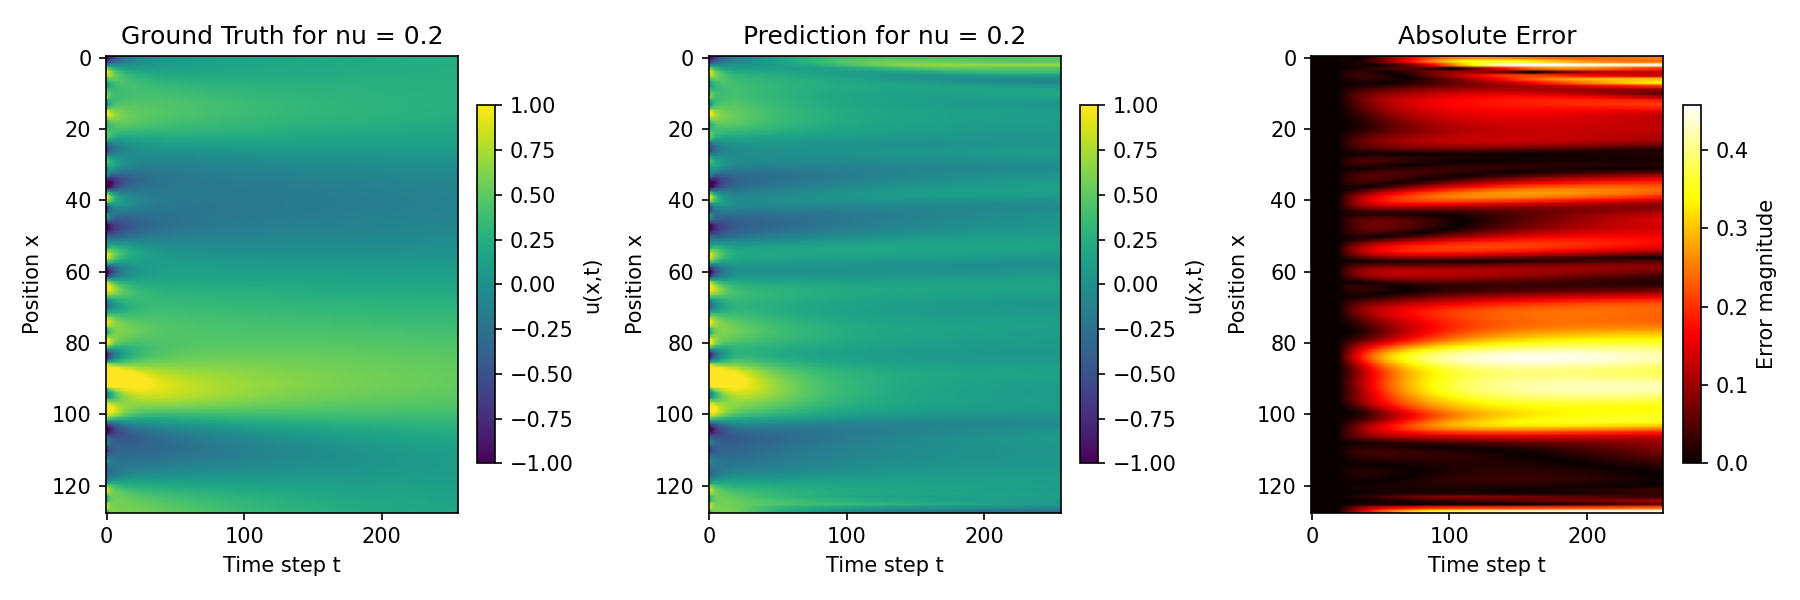
\includegraphics[width=0.48\textwidth, height=1.8cm]{images/trajectory_epoch_0_nu0.2.png}\hfill
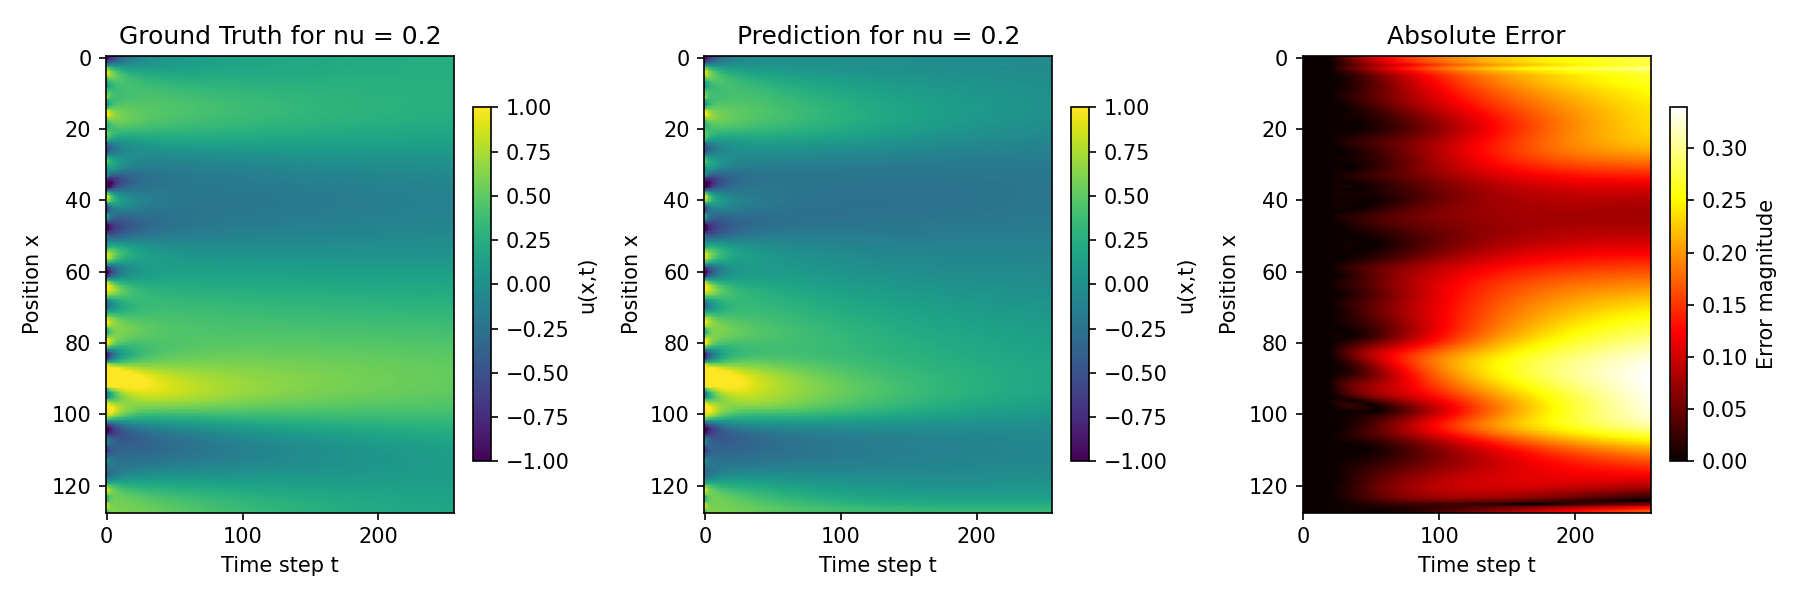
\includegraphics[width=0.48\textwidth, height=1.8cm]{images/trajectory_epoch_20_nu0.2.png}\hfill

\vspace{0.4cm}

% Row 2 (2 large subfigures)
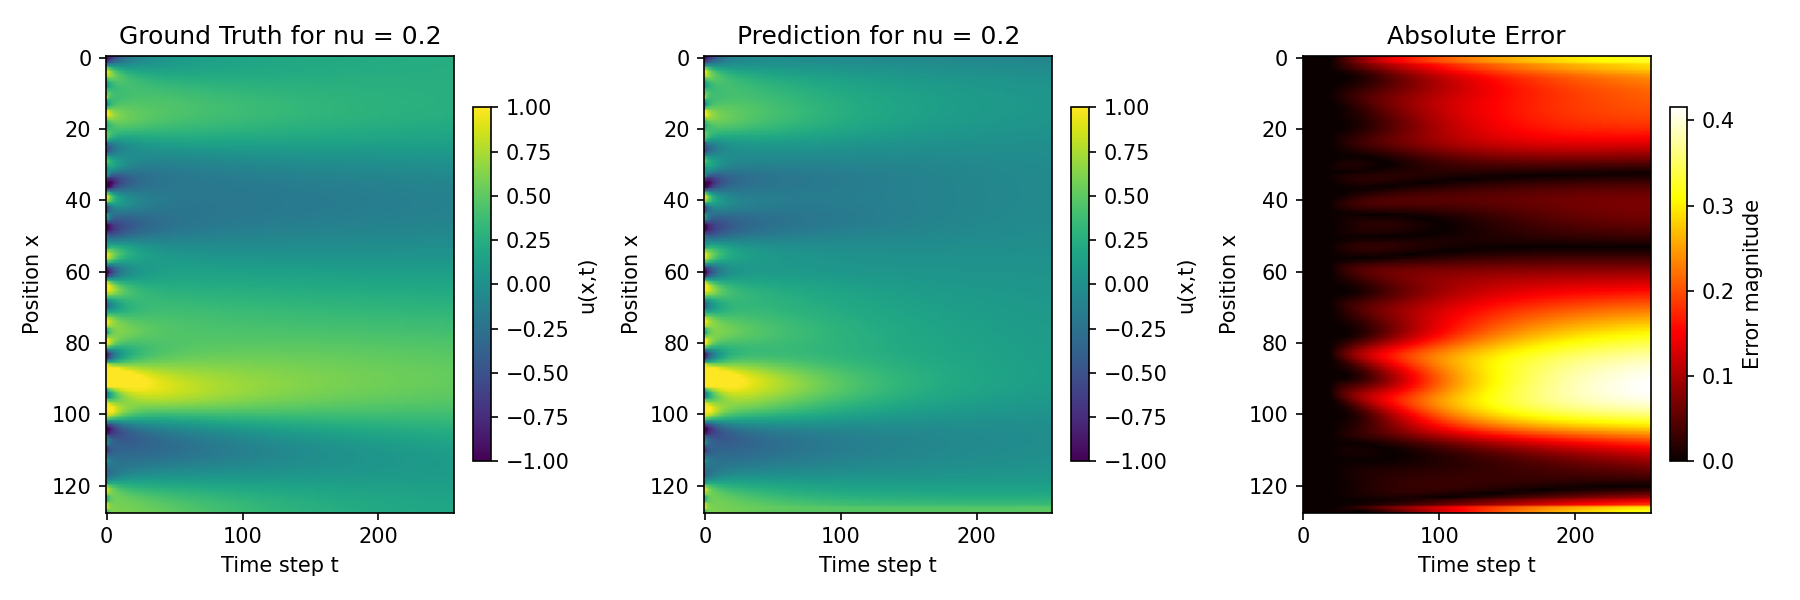
\includegraphics[width=0.48\textwidth, height=1.8cm]{images/trajectory_epoch_40_nu0.2.png}\hfill
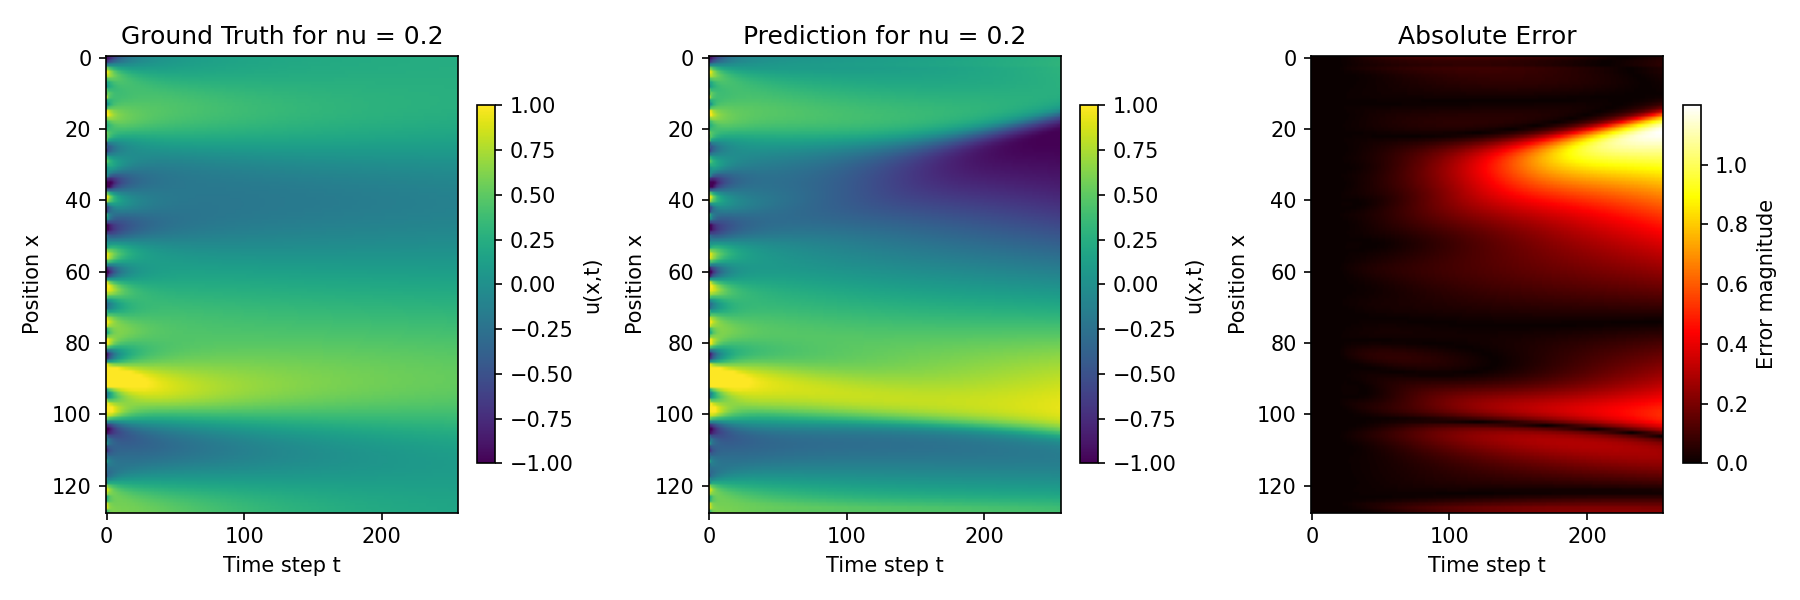
\includegraphics[width=0.48\textwidth, height=1.8cm]{images/trajectory_epoch_60_nu0.2.png}\hfill

\vspace{0.4cm}

% Row 3 (2 large subfigures)
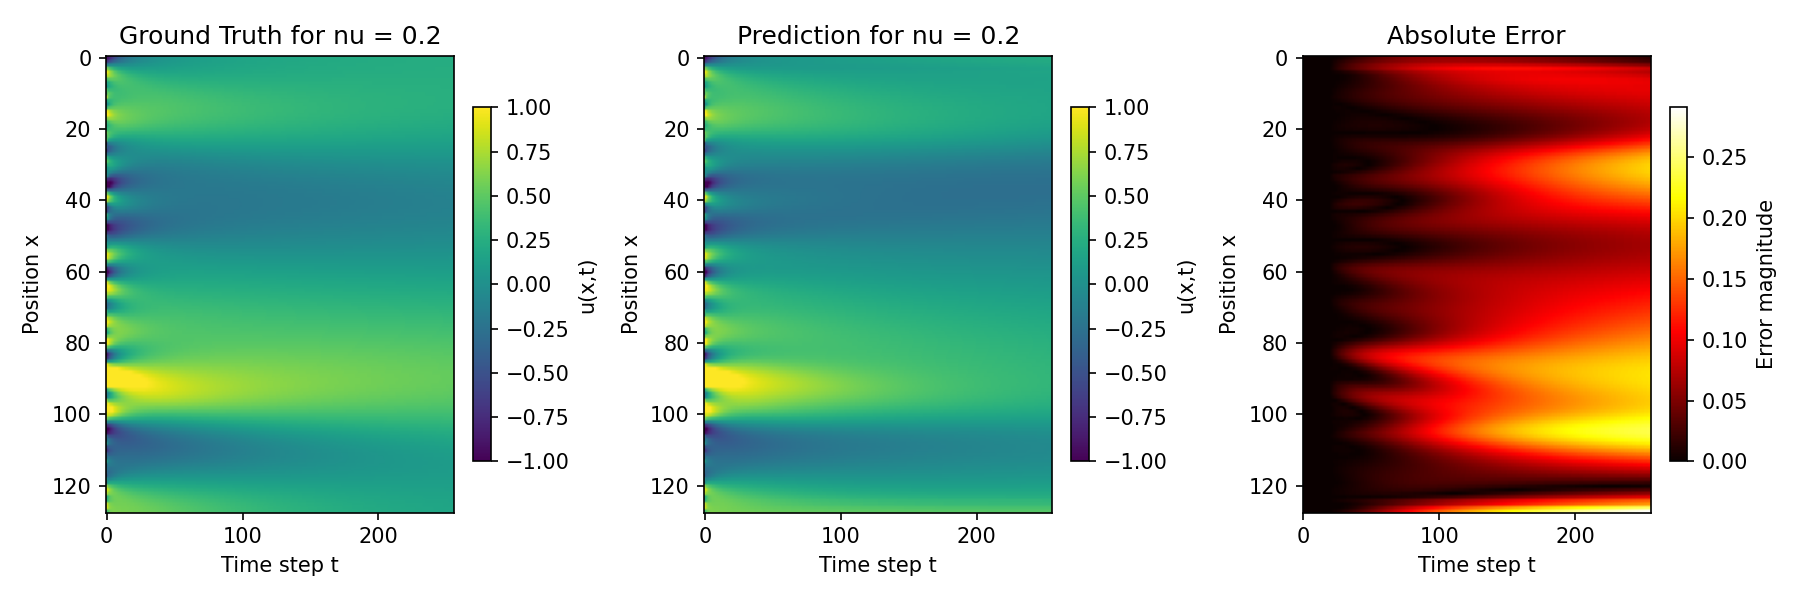
\includegraphics[width=0.48\textwidth, height=1.8cm]{images/trajectory_epoch_80_nu0.2.png}\hfill
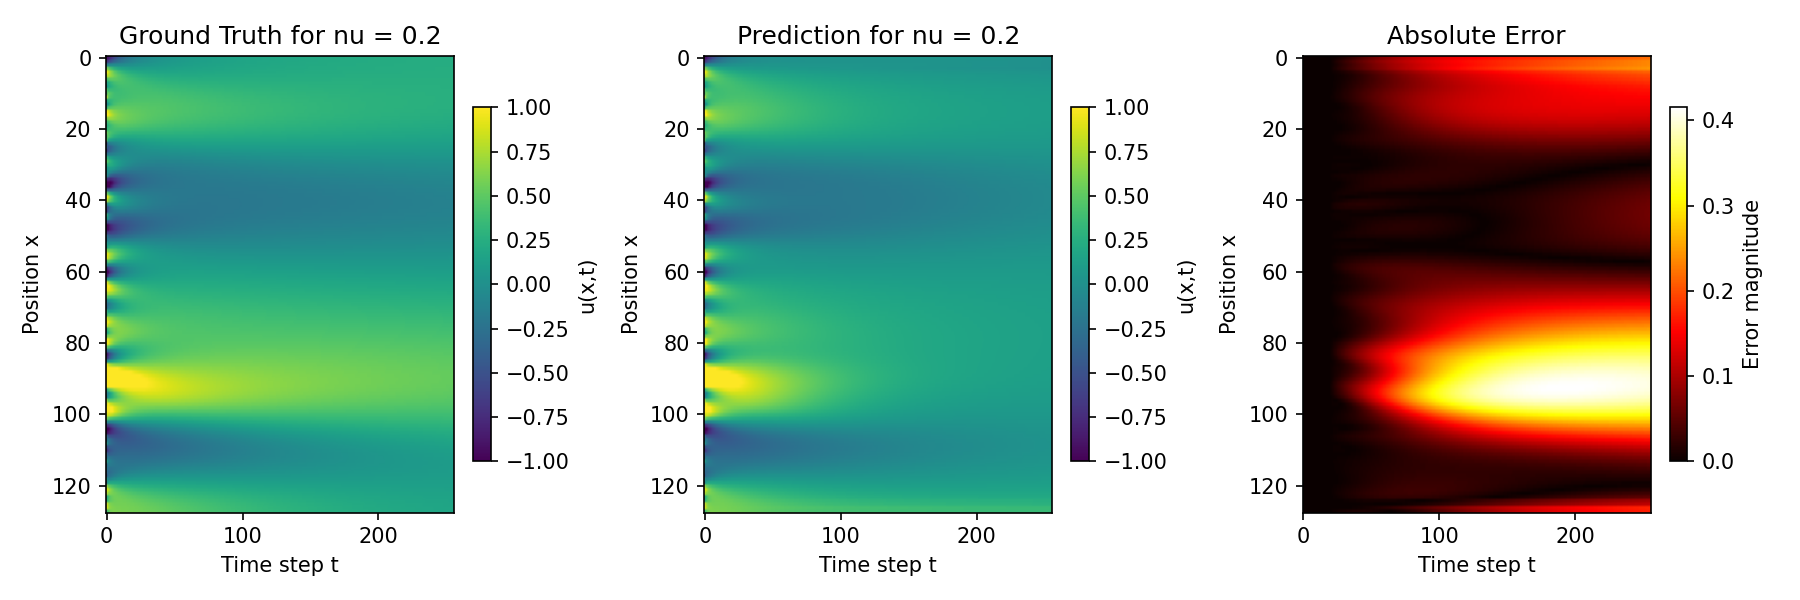
\includegraphics[width=0.48\textwidth, height=1.8cm]{images/trajectory_epoch_100_nu0.2.png}

\caption{TCAN training evolution ($\nu=0.2$). Epochs 0$\to$20 (top), 40$\to$60 (middle), 80$\to$100 (bottom).}
\label{fig:training-progress}
\end{figure}


%------------------------------ LOSS CURVE FIGURE ----------------------------

Figure~\ref{fig:loss-curve} displays the composite loss over the evaluation loop, showing steady decrease and saturation after epoch 70, confirming training stability.

\begin{figure}[h!]
\centering
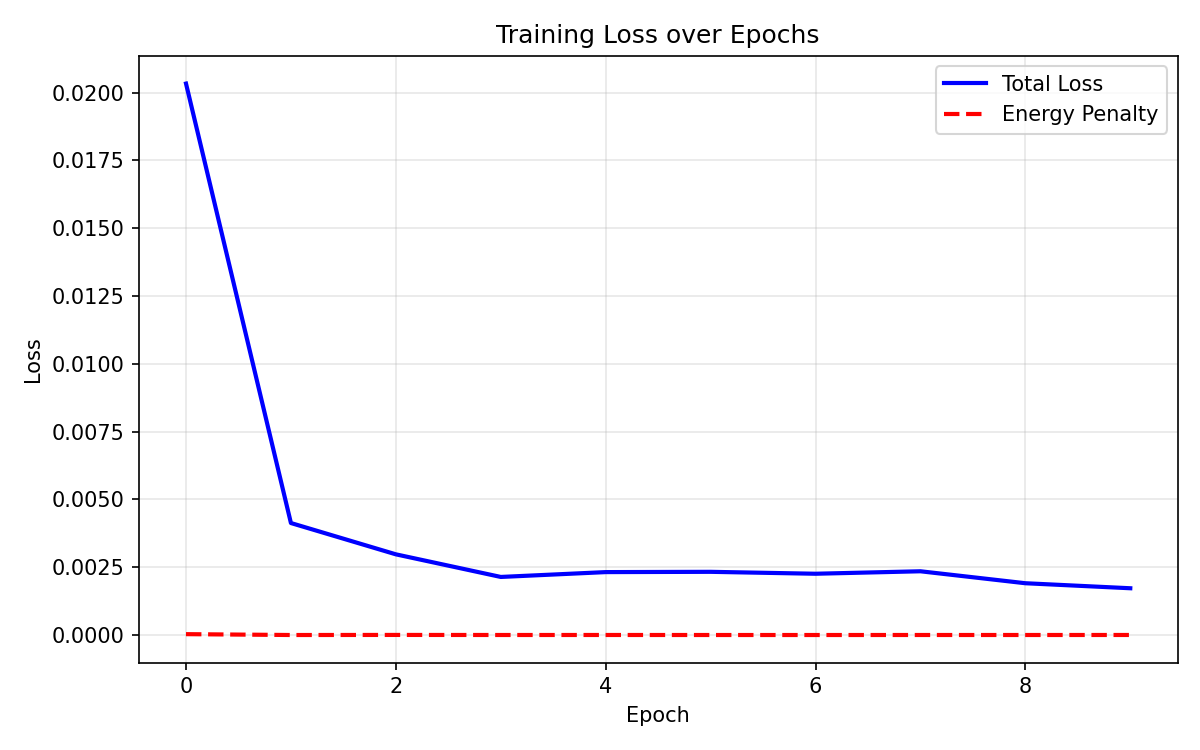
\includegraphics[width=0.6\textwidth]{images/losses_over_epochs.png}
\caption{Composite training loss ($\mathcal{L}$) over evaluation loop across 100 epochs. Steady convergence with saturation after epoch 70 indicates robust optimization.}
\label{fig:loss-curve}
\end{figure}


\paragraph{Full-trajectory results at all resolutions.}
Figure~\ref{fig:tcan-trajectories} shows TCAN autoregressive rollout predictions (after 100 training epochs) compared to ground truth for all four spatial resolutions.

\begin{figure}[h!]
  \centering
  \begin{minipage}[t]{0.48\textwidth}
    \centering
    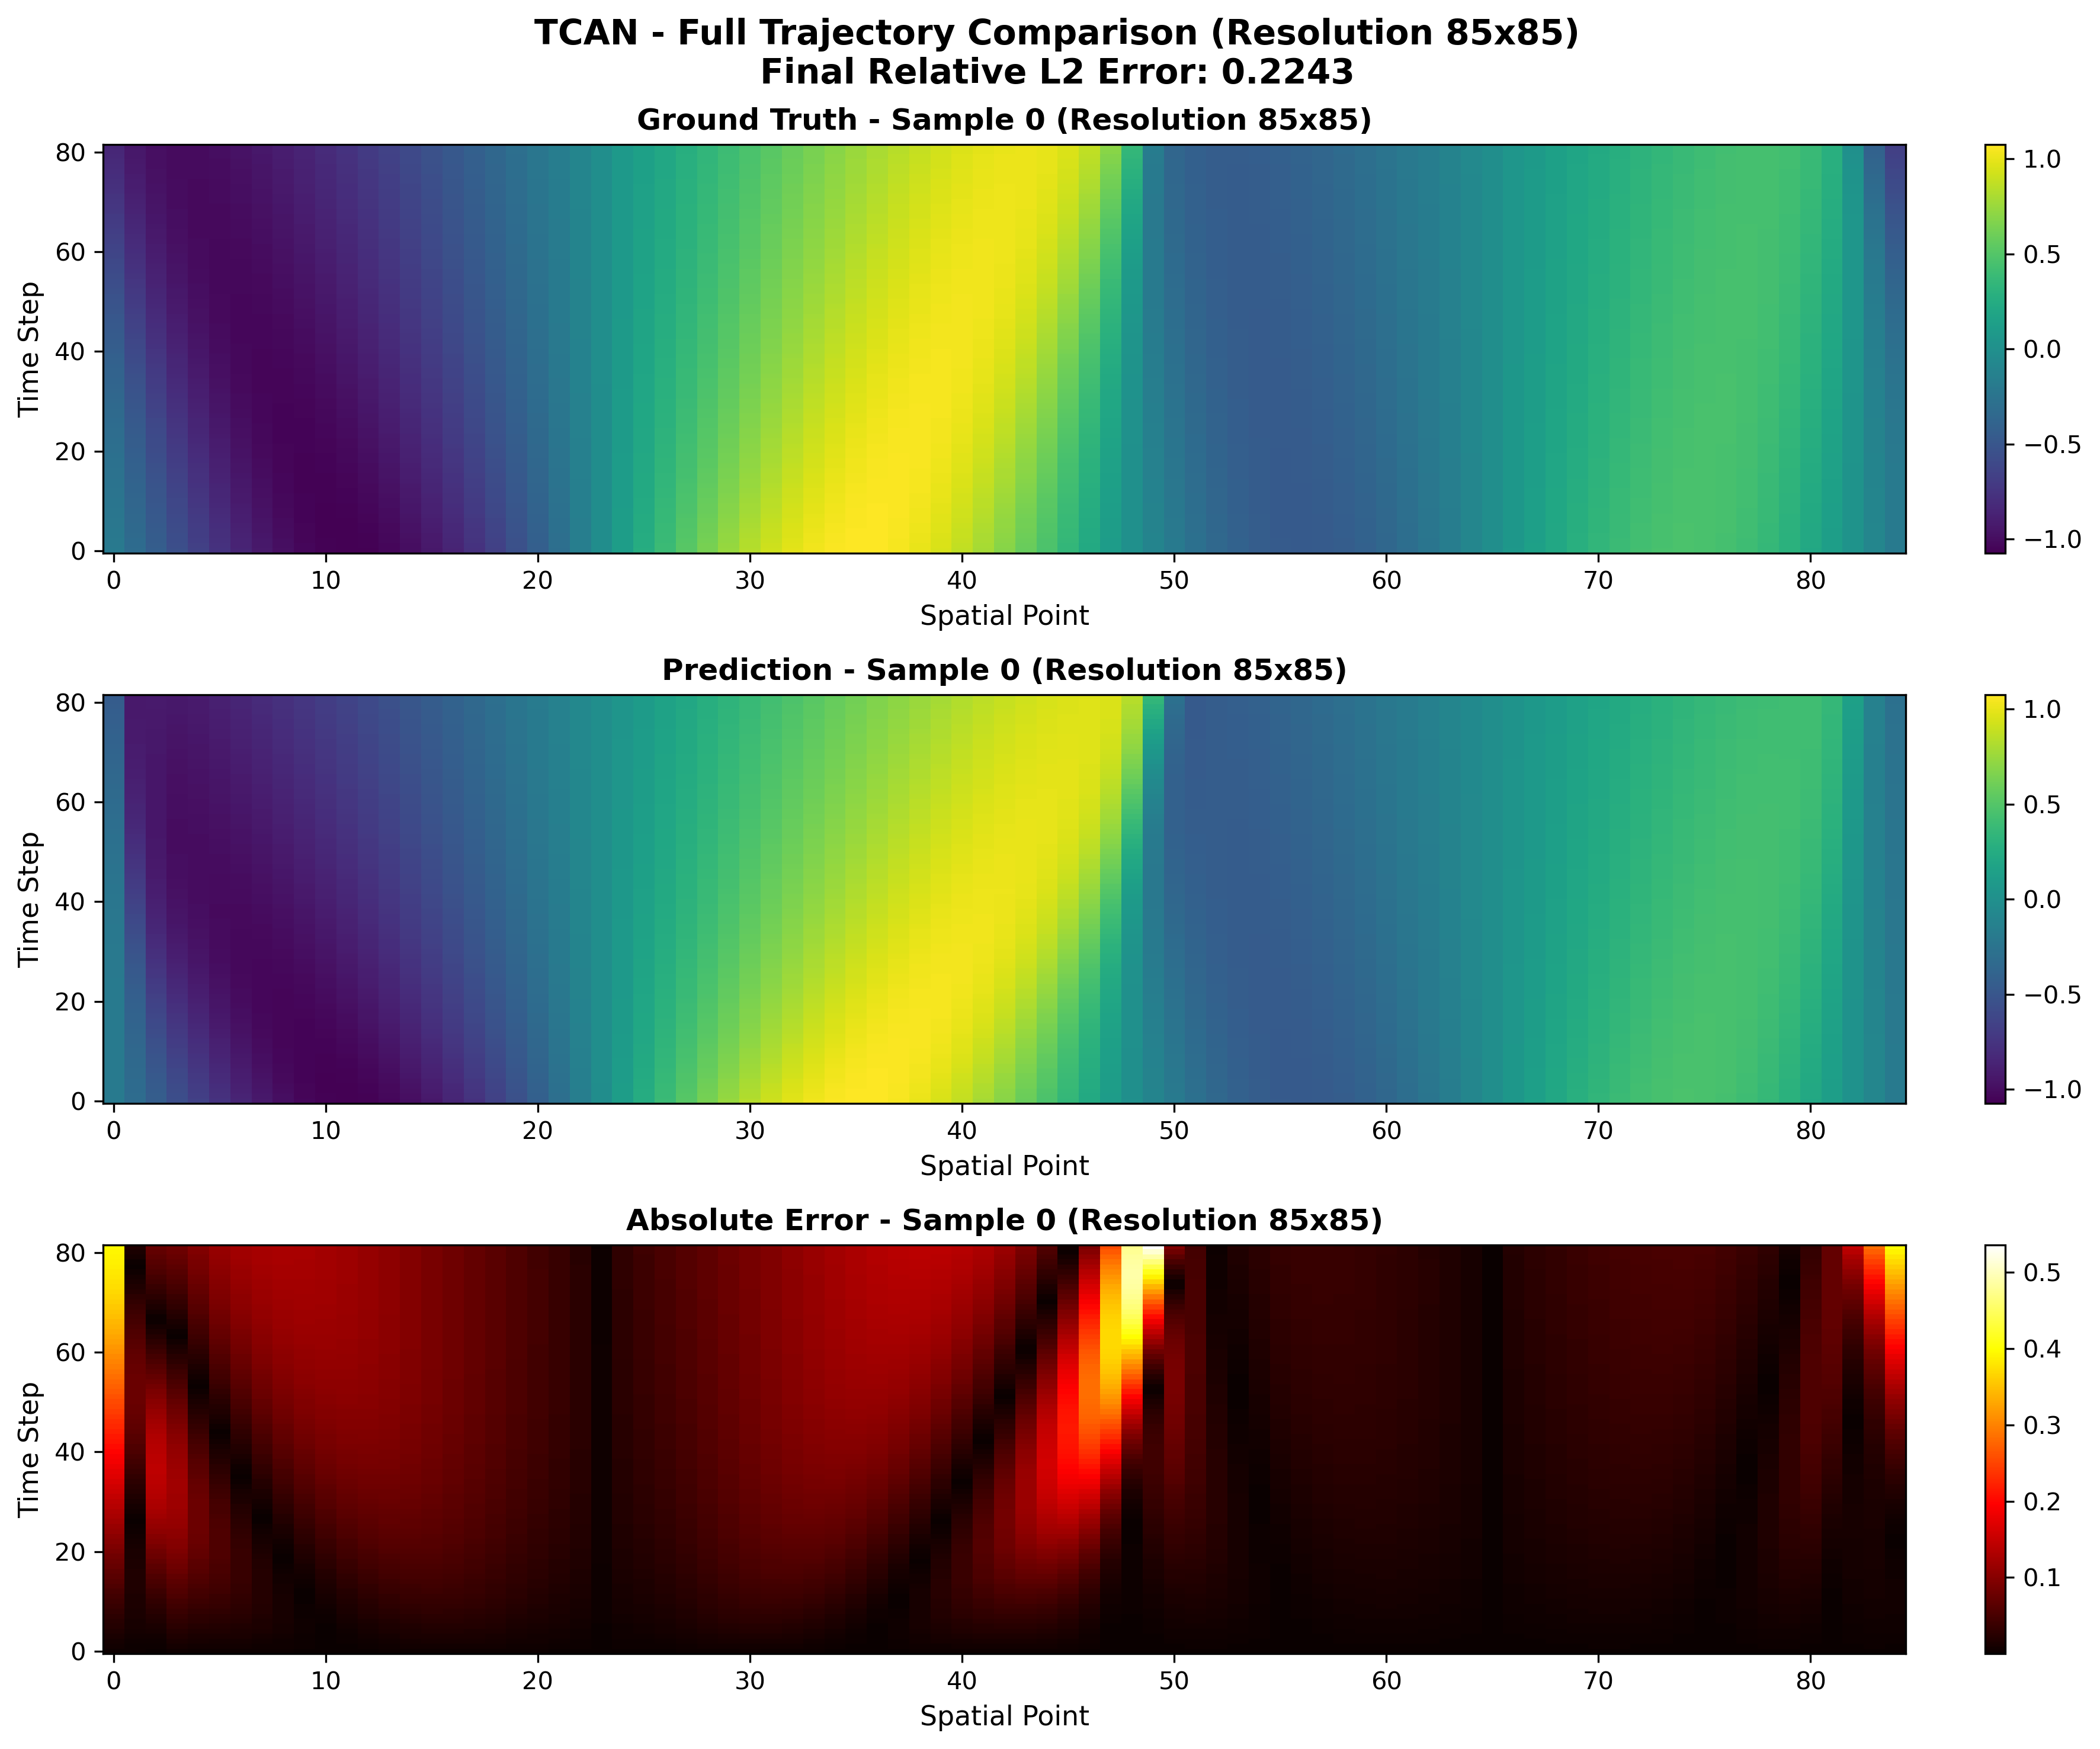
\includegraphics[width=\linewidth]{images/full_trajectory_sample_0_85x85.png}
    \caption*{$s=85$}
  \end{minipage}\hfill
  \begin{minipage}[t]{0.48\textwidth}
    \centering
    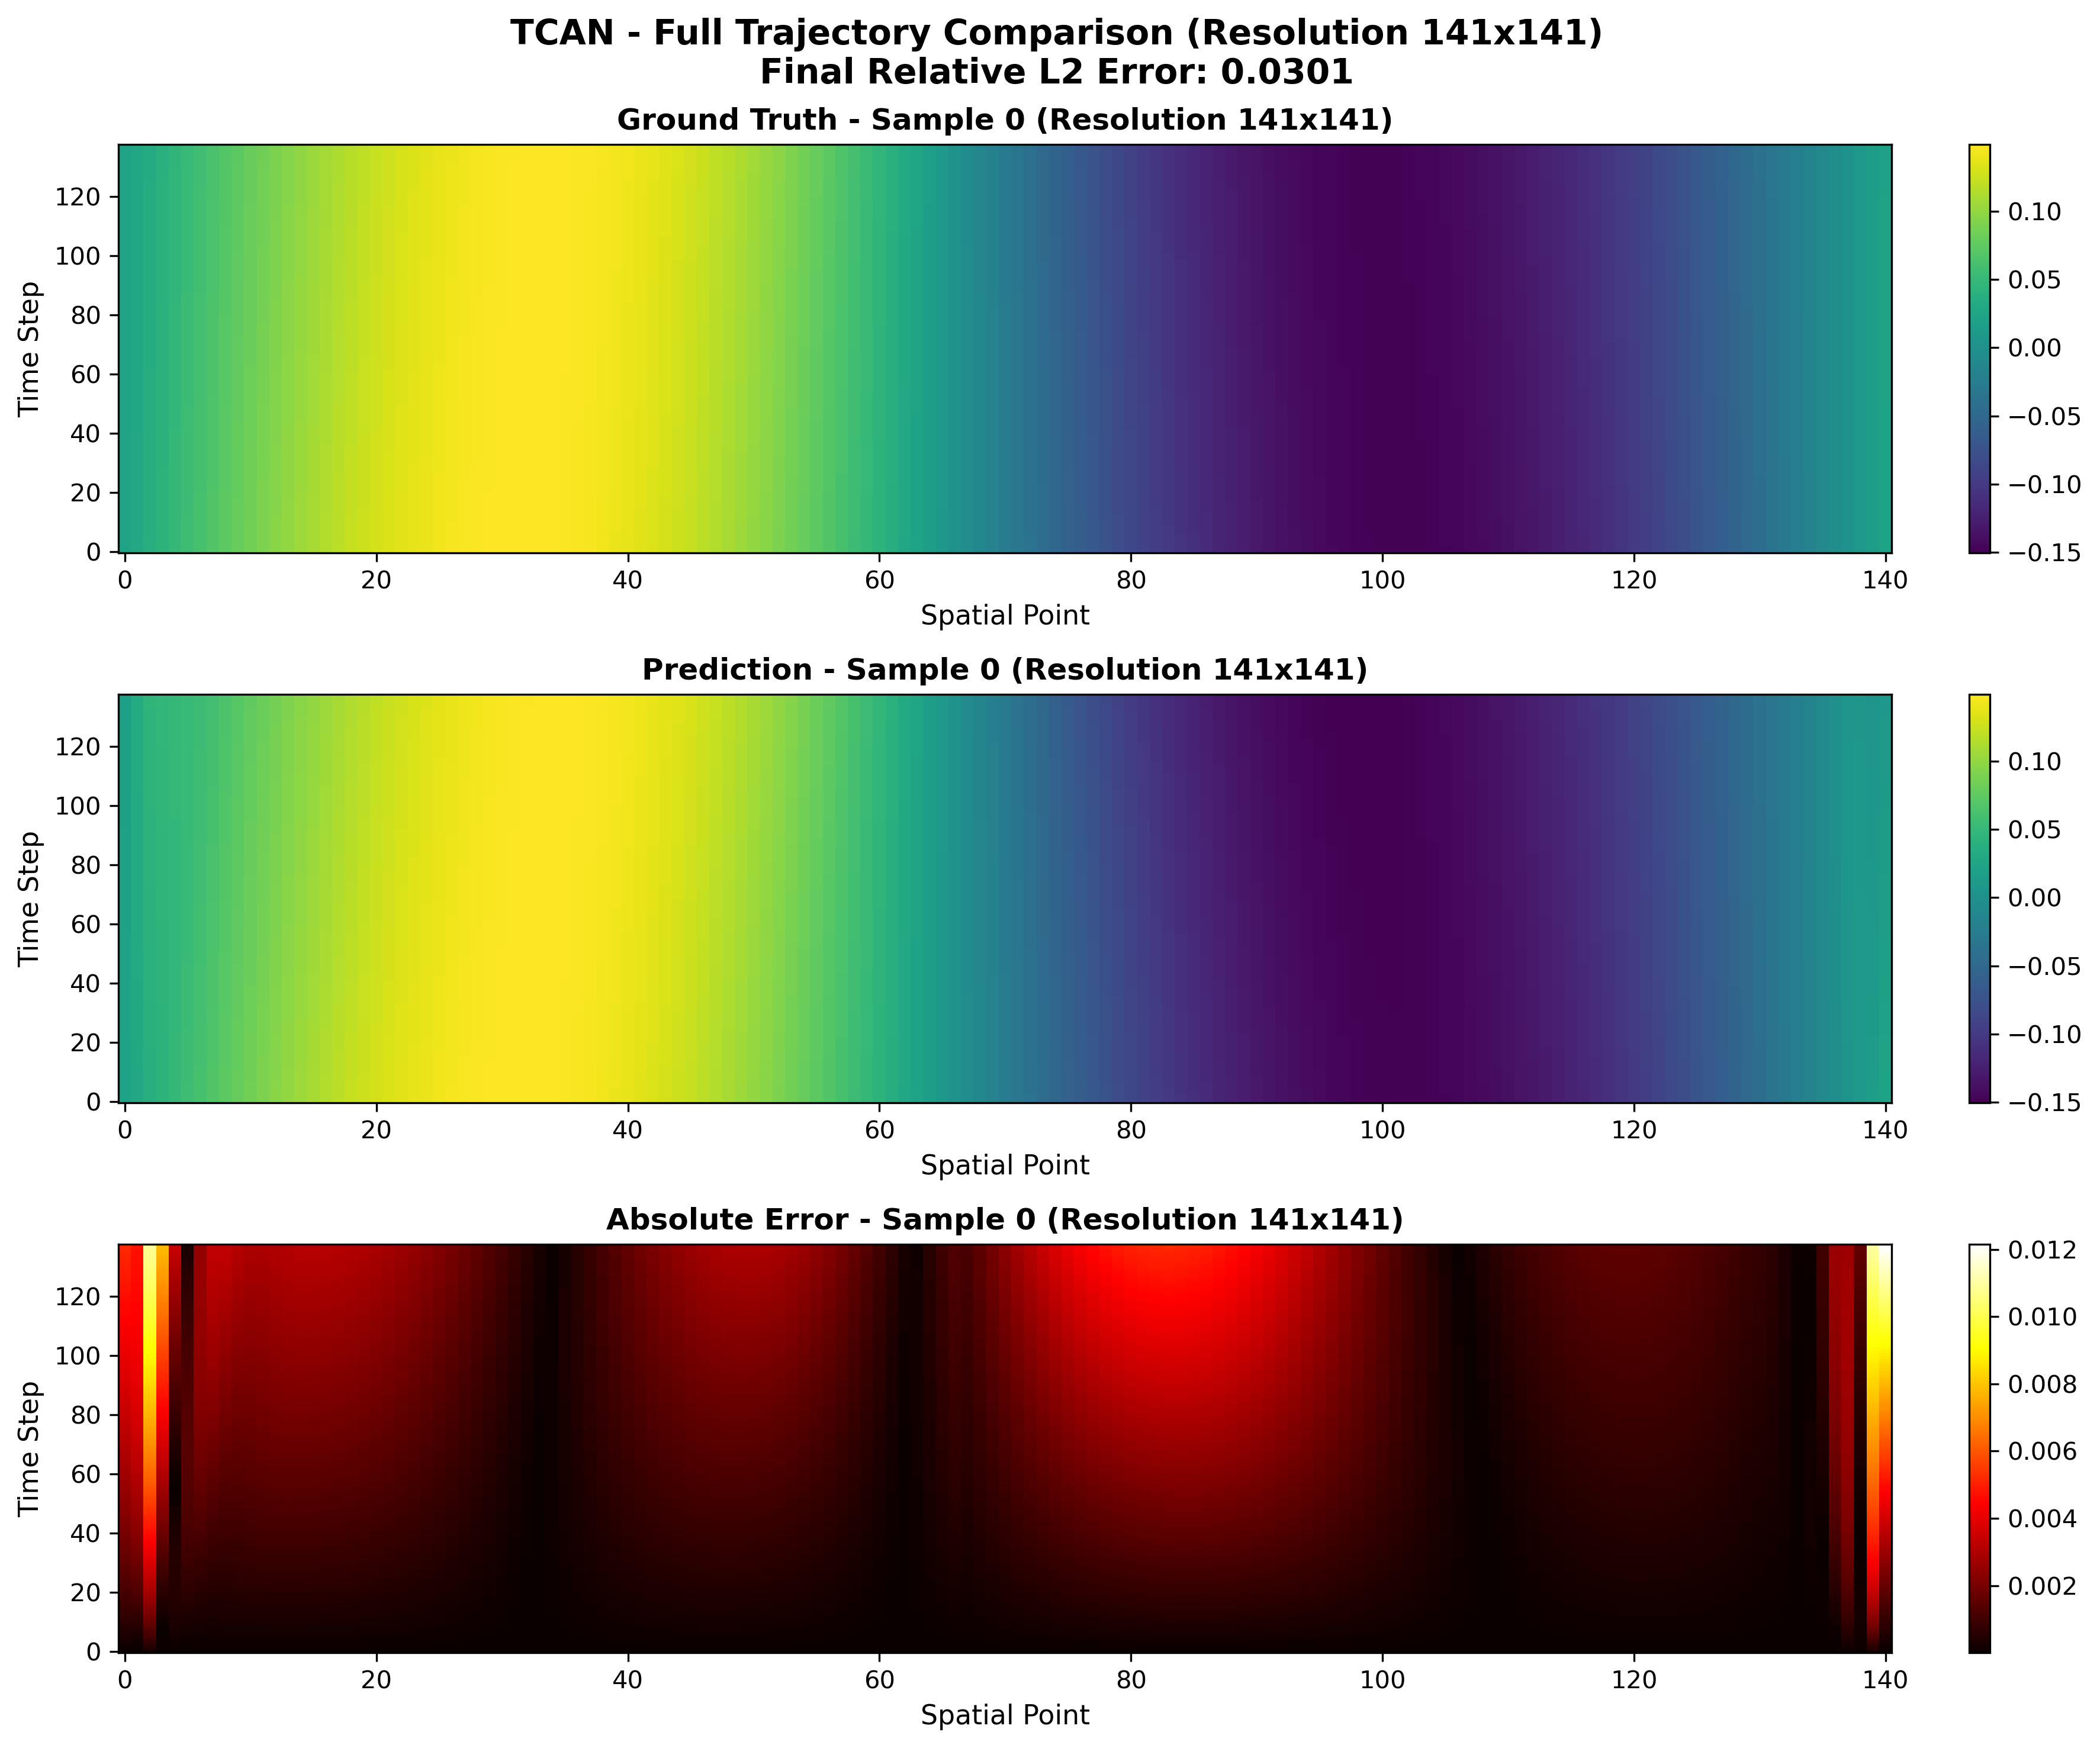
\includegraphics[width=\linewidth]{images/full_trajectory_sample_0_141x141.png}
    \caption*{$s=141$}
  \end{minipage}\\[6pt]
  \begin{minipage}[t]{0.48\textwidth}
    \centering
    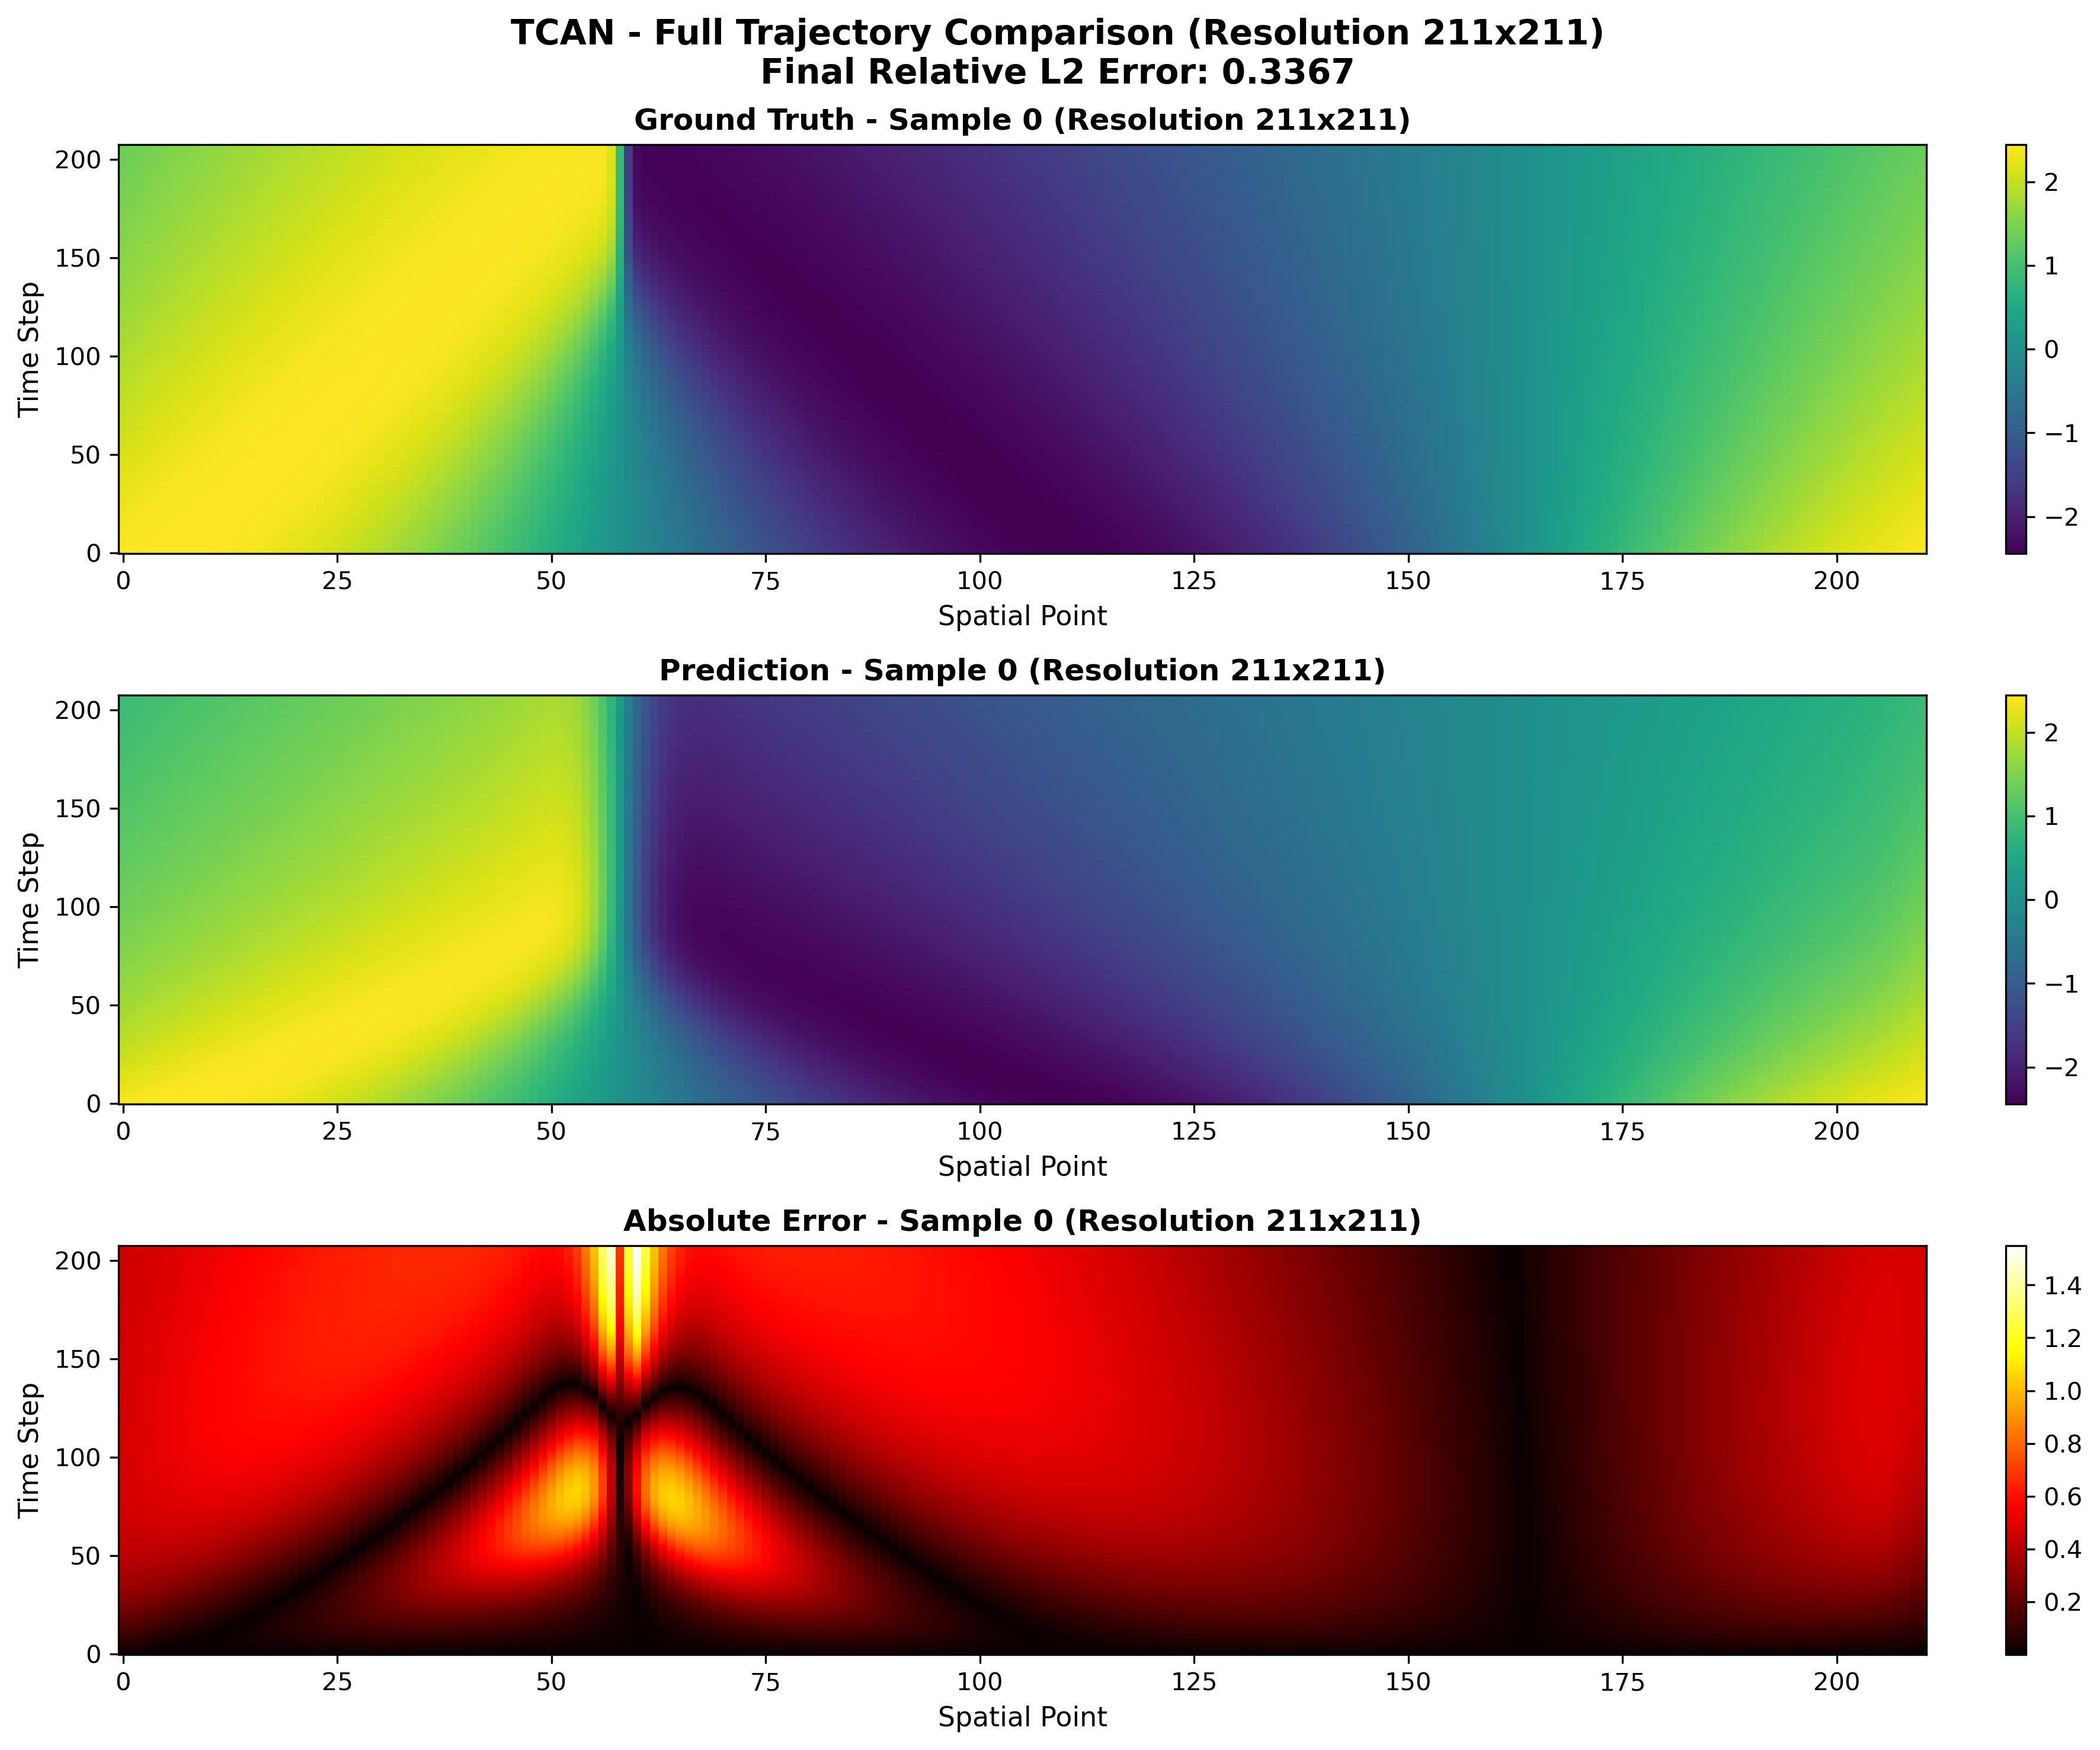
\includegraphics[width=\linewidth]{images/full_trajectory_sample_0_211x211.png}
    \caption*{$s=211$}
  \end{minipage}\hfill
  \begin{minipage}[t]{0.48\textwidth}
    \centering
    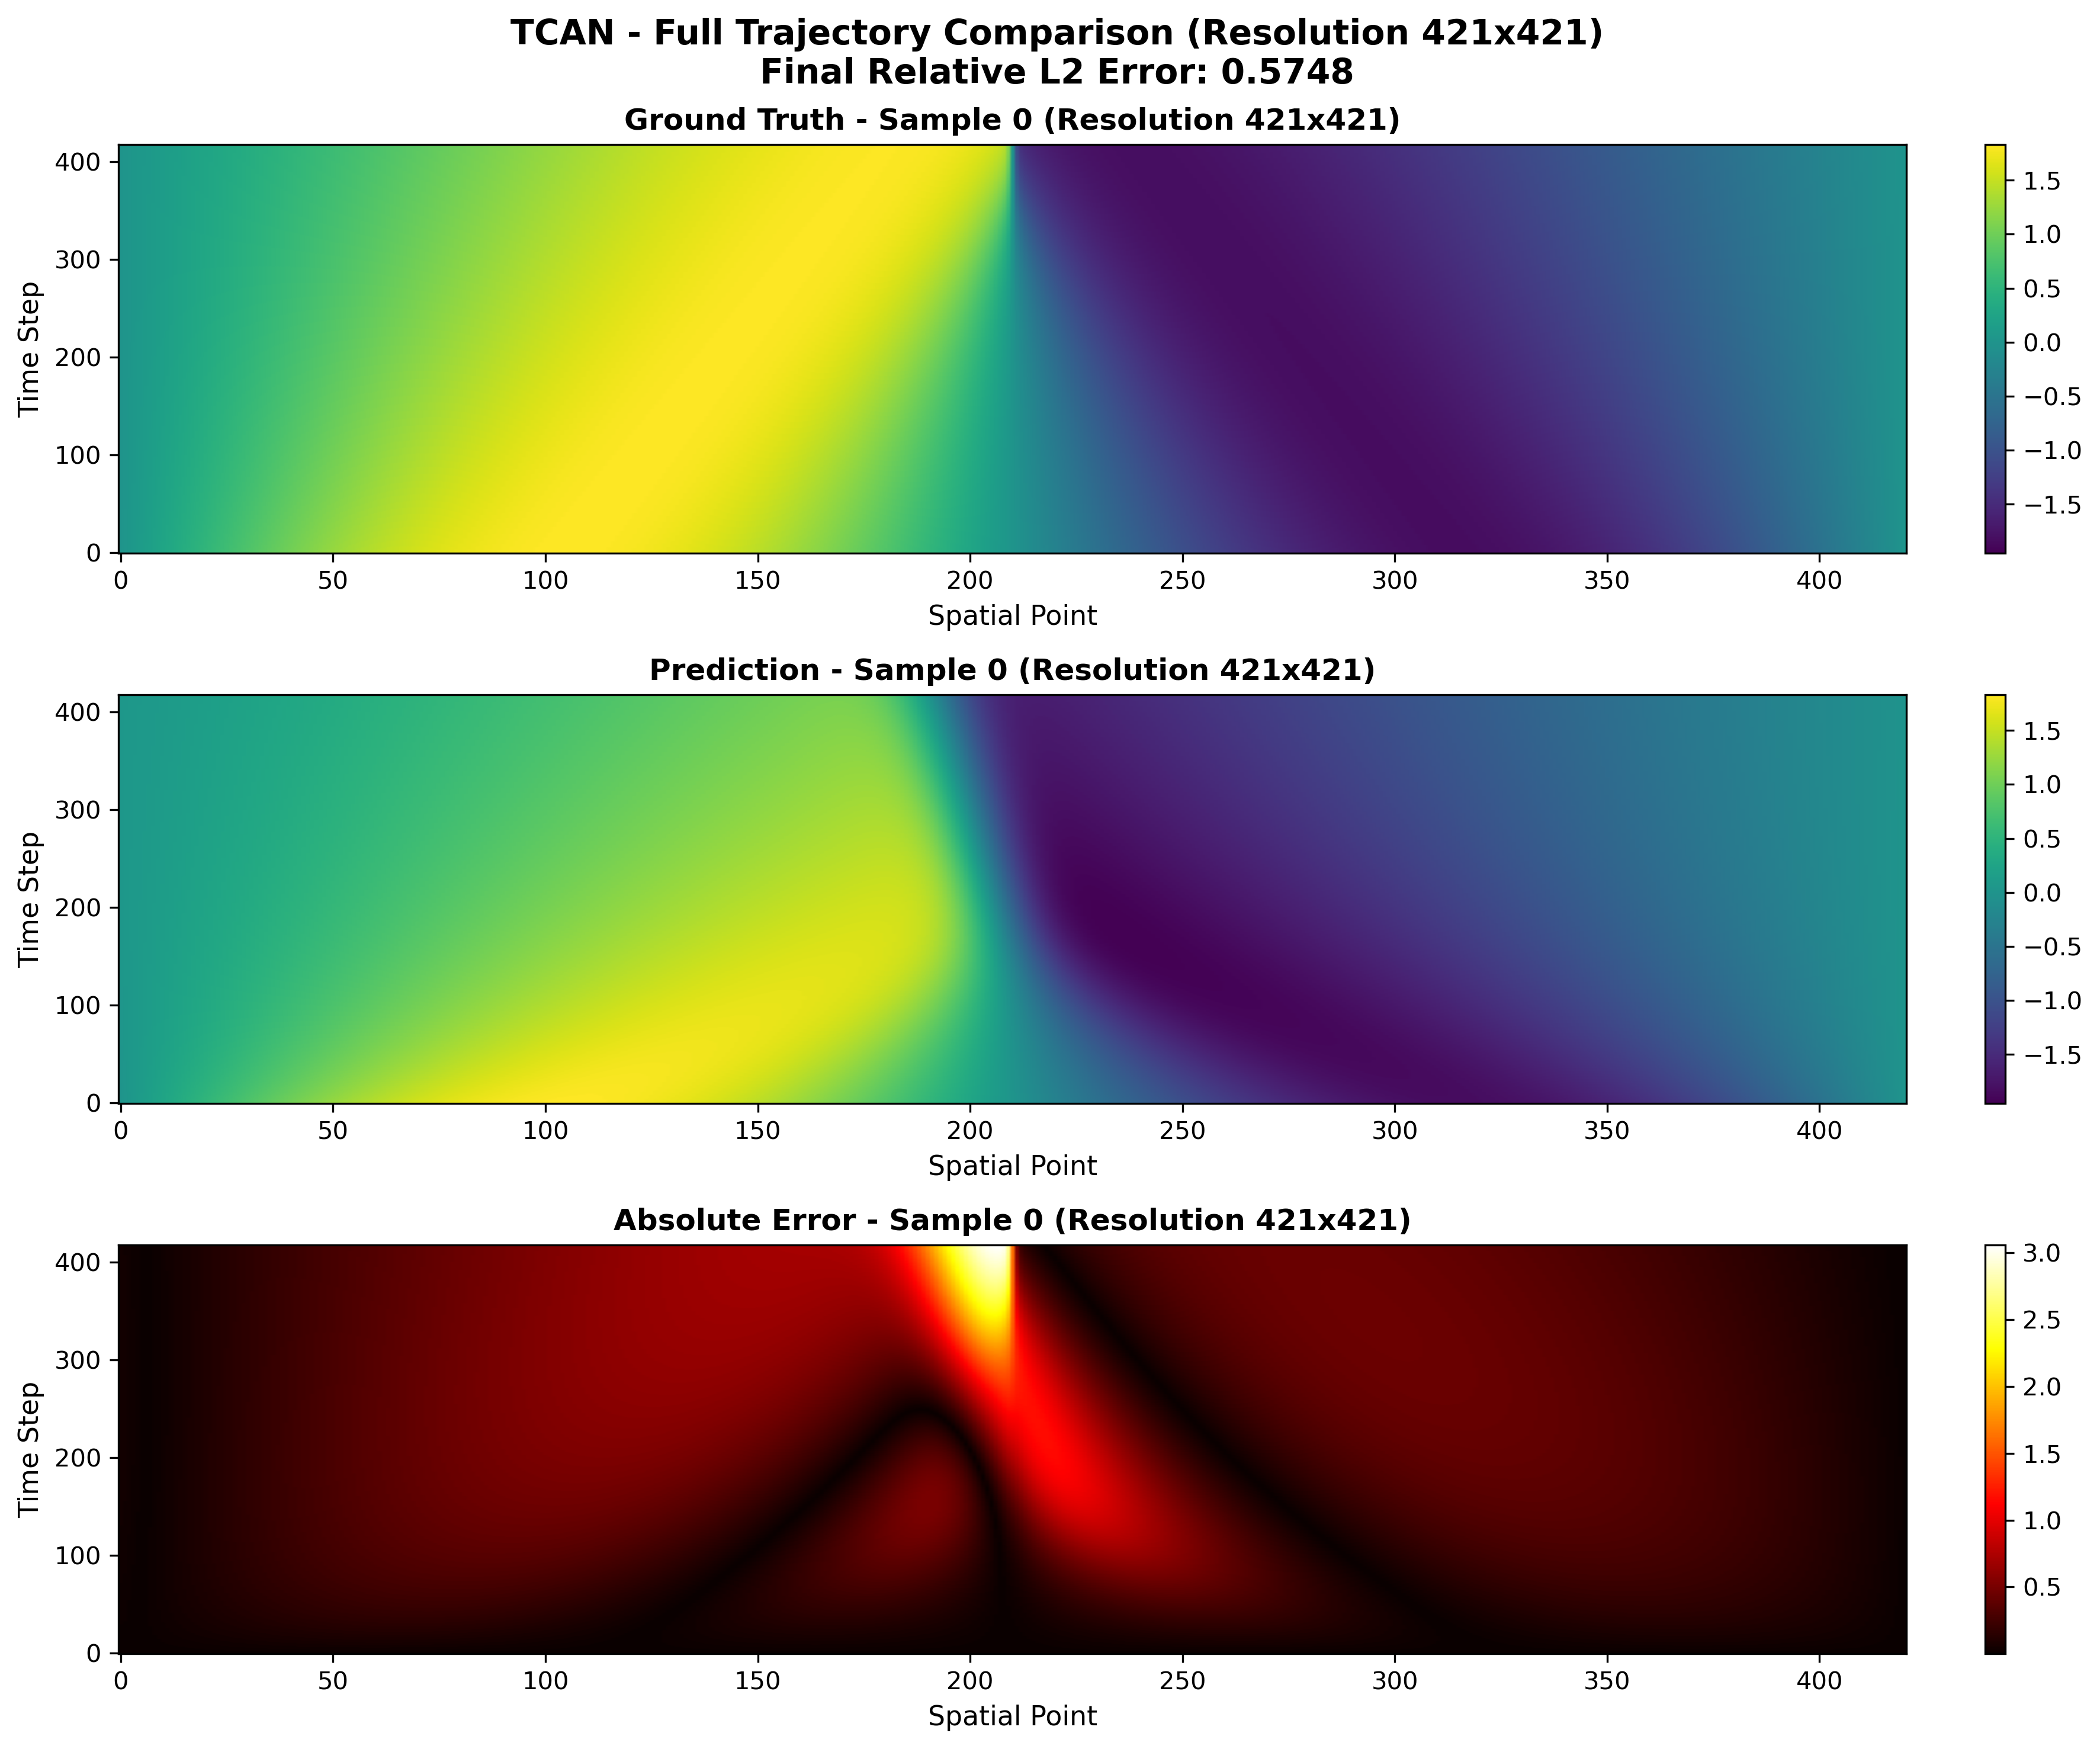
\includegraphics[width=\linewidth]{images/full_trajectory_sample_0_421x421.png}
    \caption*{$s=421$}
  \end{minipage}
  \caption{TCAN full autoregressive trajectory predictions (100 epochs) vs.~ground truth for all four spatial resolutions. Each panel shows the space-time heatmap: top half is ground truth, bottom half is the TCAN prediction. Prediction quality degrades at finer resolutions due to the longer rollout horizon.}
  \label{fig:tcan-trajectories}
\end{figure}

\subsubsection{Evaluation Metrics}
% ---------- RESULTS + EVALUATION METRICS --------------------
Full-trajectory predictions are assessed with comprehensive metrics (Table~\ref{tab:model-metrics}):

\begin{table}[h!]
\centering
\resizebox{1.1\textwidth}{!}{
\begin{tabular}{@{\extracolsep{14pt}}l@{\extracolsep{14pt}}c@{\extracolsep{14pt}}l@{\extracolsep{14pt}}c@{\extracolsep{14pt}}c}
\toprule
\textbf{Metric} & \textbf{Formula} & \textbf{Purpose} & \textbf{Good} & \textbf{Failure} \\
\midrule[1pt]
MSE & $\frac{1}{NP}\sum(u_\text{pred}-u_\text{gt})^2$ & Pixel accuracy & $<10^{-4}$ & $>10^{-3}$ \\
Rel. $L^2$ & $\|u_\text{pred}-u_\text{gt}\|_2/\|u_\text{gt}\|_2$ & Scale-invariant & $<0.05$ & $>0.2$ \\
PSNR & $20\log(\text{range}/\sqrt{\text{MSE}})$ & Image quality & $>30$dB & $<20$dB \\
SSIM & Structural similarity & Texture preservation & $>0.9$ & $<0.7$ \\
Correlation & Pearson $r$/step & Phase alignment & $>0.95$ & $<0.8$ \\
\hline[0.8pt]
Mass Error & $|\int u\,dx-M_0|$ & Conservation & $<0.01$ & $>0.1$ \\
Energy Monotonicity & $E(t+1)\leq E(t)$ & Dissipation & $>0.95$ & $<0.8$ \\
PDE Residual & $\|F(u)\|_2$ & PDE satisfaction & $<0.01$ & $>0.1$ \\
Max Gradient & $\max|\partial_xu|$ & Shock preservation & $\pm10\%$GT & Diverges \\
Gradient Error & $\|\nabla_x(u_\text{pred}-u_\text{gt})\|_2$ & Shock sharpness & $<0.05$ & $>0.2$ \\
\bottomrule[1pt]
\end{tabular}
}
\caption{TCAN evaluation metrics with formulas, purposes, and thresholds.}
\label{tab:model-metrics}
\end{table}

\subsubsection{Comparison Against FNO}

Table~\ref{tab:tcan-vs-fno} reports the relative $L^2$ error of TCAN against the Fourier Neural Operator~\cite{li2021fourier} across all four spatial resolutions of the benchmark dataset.

\begin{table}[h!]
\centering
\begin{tabular}{lcccc}
\toprule
\textbf{Method} & $s=85$ & $s=141$ & $s=211$ & $s=421$ \\
\midrule
FNO~\cite{li2021fourier} & \textbf{0.0108} & \textbf{0.0109} & \textbf{0.0109} & \textbf{0.0098} \\
TCAN (ours)              & 0.303  & 0.335  & 0.726  & 0.944  \\
\bottomrule
\end{tabular}
\caption{Relative $L^2$ error on the 1D Burgers FNO benchmark at four spatial resolutions. Lower is better. FNO errors are taken directly from~\cite{li2021fourier}; TCAN errors are from our experiments.}
\label{tab:tcan-vs-fno}
\end{table}

\paragraph{Why FNO achieves lower error.}
FNO~\cite{li2021fourier} is a \emph{single-step operator}: given the initial condition $u_0(\cdot)$, it directly predicts the solution $u(\cdot, T=1)$ in a single forward pass through four Fourier layers. Because the Fourier integral kernel has a global spatial receptive field (acting on all $k_{\max}=16$ Fourier modes simultaneously), FNO captures the long-range correlations present in Burgers dynamics without any temporal unrolling. Its relative $L^2$ error stays below $1.1 \times 10^{-2}$ across all resolutions, and it is essentially unaffected by spatial resolution since the learned weight tensor $R_\ell$ acts on Fourier coefficients rather than grid points.

\paragraph{The autoregressive gap.}
TCAN, by contrast, calls the controller once per time step and rolls out up to 256 steps to reach $T=1$. Small per-step prediction errors compound multiplicatively: if the one-step error is $\epsilon$, the error after $T$ steps grows as $O(\epsilon T)$ or worse near shocks. This explains the monotonic degradation from $0.30$ at $s=85$ (fewer rollout steps) to $0.94$ at $s=421$ (more rollout steps). The $\times 28$ gap at $s=85$ between FNO and TCAN is therefore attributable primarily to the one-step versus autoregressive formulation, not to the choice of spatial architecture.
\chapter{Extension to 2D Burgers Equation}
\label{chap:2d}

The 1D viscous Burgers equation served as a first testbed to validate the NFTM framework with a TCAN controller. Extending to two spatial dimensions is a necessary step toward realistic applications: flow over a wing, wake dynamics around a car, or heat transport in planar geometries all require at least two dimensions to capture the essential physics. This chapter describes the 2D dataset we generated, the architecture modifications required for 2D input, the preliminary training results, and the lessons learned that will inform the subsequent extension to incompressible Navier-Stokes.

%==============================================================================
\section{Two-Dimensional Burgers Equation}
\label{sec:2d_burgers_equation}
%==============================================================================

The two-dimensional viscous Burgers equation is a natural extension of the 1D case and retains many of its key features: nonlinear advection, viscous diffusion, and shock formation. It is written as a coupled system for the two velocity components $u(x,y,t)$ and $v(x,y,t)$:

\begin{align}
  \frac{\partial u}{\partial t} + u\frac{\partial u}{\partial x} + v\frac{\partial u}{\partial y}
  &= \nu\left(\frac{\partial^2 u}{\partial x^2} + \frac{\partial^2 u}{\partial y^2}\right),
  \label{eq:2d_burgers_u} \\[6pt]
  \frac{\partial v}{\partial t} + u\frac{\partial v}{\partial x} + v\frac{\partial v}{\partial y}
  &= \nu\left(\frac{\partial^2 v}{\partial x^2} + \frac{\partial^2 v}{\partial y^2}\right),
  \label{eq:2d_burgers_v}
\end{align}

on a periodic domain $(x,y)\in[0,1]^2$ with viscosity $\nu > 0$. Compared to the 1D case, the coupling of the two components and the richer spatial structure of the 2D field make this a substantially more demanding learning problem.

%==============================================================================
\section{Dataset Generation}
\label{sec:2d_dataset}
%==============================================================================

A custom dataset of 2D Burgers trajectories was generated by numerically solving the system (\ref{eq:2d_burgers_u})--(\ref{eq:2d_burgers_v}) for varying viscosity values $\nu$. The initial conditions for both $u_0(x,y)$ and $v_0(x,y)$ were drawn from a random Gaussian field, following the same strategy as the 1D FNO dataset (Section~\ref{sec:data-generation}).

Each trajectory was discretized on a spatial grid of size $H \times W = 64 \times 64$ and integrated over $T = 64$ time steps, yielding snapshots of shape $(2, H, W)$ (one channel per velocity component). The viscosity was sampled uniformly: $\nu \sim \mathcal{U}(0.005, 0.5)$, spanning both near-inviscid shock regimes and smoothly diffusive flows.

\begin{figure}[h!]
  \centering
  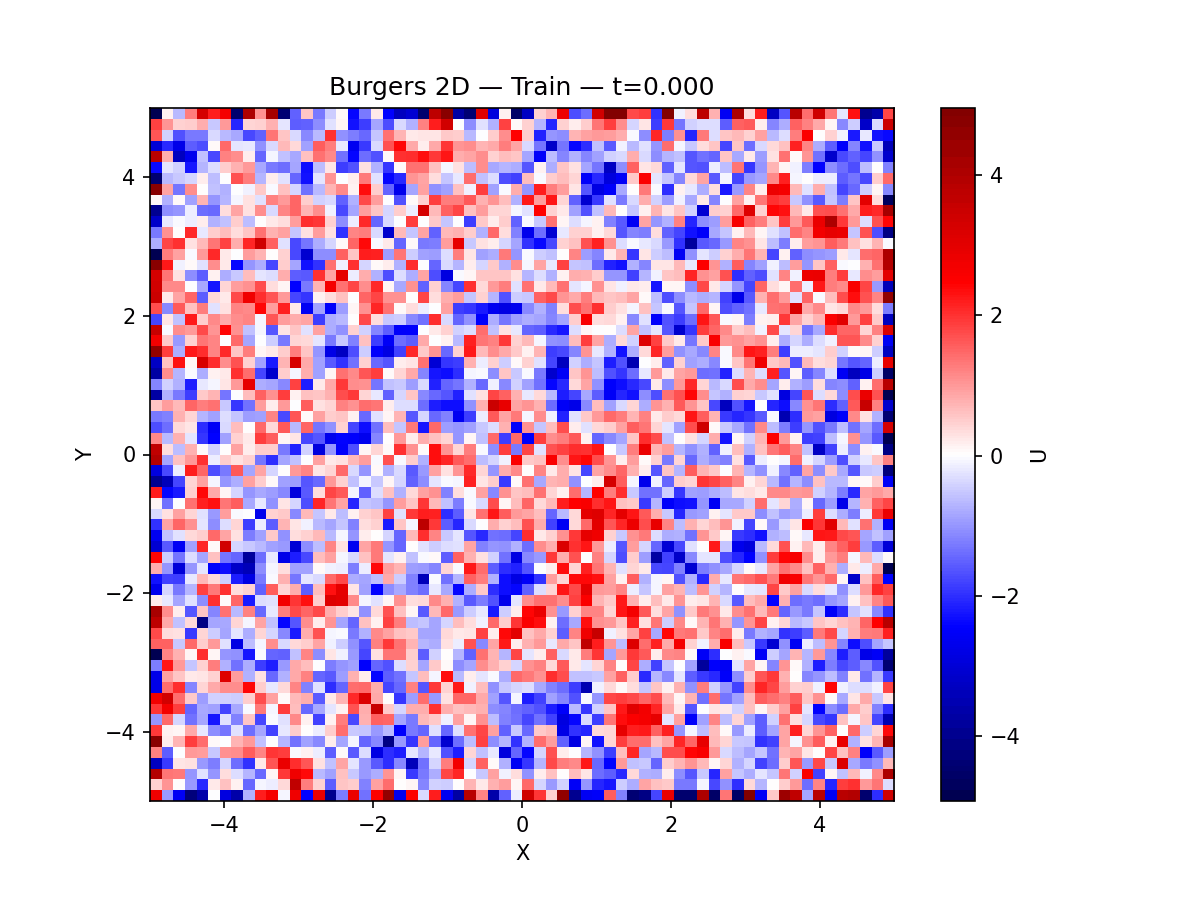
\includegraphics[width=0.72\textwidth]{images/2D_train_sample.png}
  \caption{Representative training sample from the 2D Burgers dataset ($\nu=0.05$, $64\times64$ grid). Each row shows one velocity component ($u$ top, $v$ bottom) at successive time steps. The diagonal shock structure illustrates the coupled 2D dynamics that the model must learn to reproduce autoregressively.}
  \label{fig:2d-train-sample}
\end{figure}

%==============================================================================
\section{Model Architecture}
\label{sec:2d_architecture}
%==============================================================================

The 2D model is derived from the 1D TCAN controller (Chapter~\ref{chap:approaches}) by replacing all 1D spatial operations with their 2D counterparts. The overall pipeline is identical: the model receives a history window of $W$ past fields and predicts the next field in an autoregressive rollout.

\paragraph{Input.}
The history window is a tensor of shape $(B, W, C, H, W_{\text{grid}})$, where $B$ is the batch size, $W$ is the number of past time steps, $C=2$ is the number of channels (velocity components), and $H \times W_{\text{grid}}$ is the spatial resolution.

\paragraph{Causal Temporal Attention (2D).}
As in the 1D case, a causal attention mechanism assigns learned importance weights to each past time step, restricting attention to the past. Spatial features at each time step are extracted with shared 2D convolutional layers before attention is computed.

\paragraph{FiLM Conditioning.}
The viscosity $\nu$ is injected as a scalar via a Feature-wise Linear Modulation (FiLM) layer, allowing the same weights to handle the full viscosity range.

\paragraph{Conv2D Decoder and Residual Correction.}
A stack of 2D convolutional layers maps the context vector back to a spatial field. The model predicts a bounded residual $\Delta u$, clipped via a tanh activation:
\[
  \hat{u}_{t+1} = u_t + \tanh\!\bigl(\Delta u_{\theta}(u_{t-W+1:t},\, \nu)\bigr).
\]
This residual formulation improves numerical stability during long rollouts. The complete pipeline is:
\[
  \underbrace{(B,W,C,H,W_{\text{grid}})}_{\text{History window}}
  \xrightarrow{\text{Causal Attn (2D)}}
  \xrightarrow{\text{FiLM}(\nu)}
  \xrightarrow{\text{Conv2D decoder}}
  \xrightarrow{\tanh\,\Delta}
  \underbrace{\hat{u}_{t+1}}_{\text{Next field}}.
\]

%==============================================================================
\section{Preliminary Results}
\label{sec:2d_results}
%==============================================================================

Training proceeded successfully in the sense that both training and validation losses decreased monotonically, confirming that gradient flow and optimization are stable for the 2D architecture. However, the model's spatial predictions remain qualitatively poor: it fails to reproduce the correct field structures and produces systematic low-frequency artifacts.

\begin{figure}[h!]
  \centering
  \begin{minipage}[t]{0.47\textwidth}
    \centering
    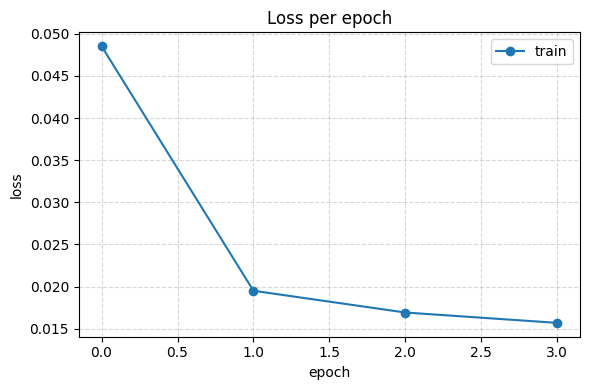
\includegraphics[width=\linewidth]{images/2D_loss.png}
    \caption{Training and validation loss curves for the 2D TCAN model over 100 epochs. Both curves decrease monotonically, confirming stable optimisation.}
    \label{fig:2d-loss}
  \end{minipage}\hfill
  \begin{minipage}[t]{0.47\textwidth}
    \centering
    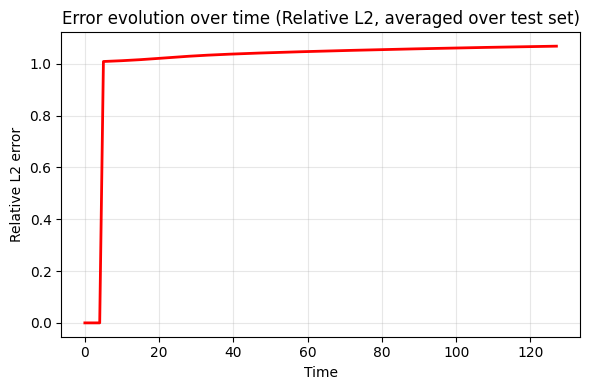
\includegraphics[width=\linewidth]{images/2D_output.png}
    \caption{Sample prediction from the 2D TCAN model after 100 epochs. Despite stable training, the predicted field (right) fails to reproduce the spatial structure of the ground truth (left), highlighting the remaining performance gap.}
    \label{fig:2d-output}
  \end{minipage}
\end{figure}

\begin{figure}[h!]
  \centering
  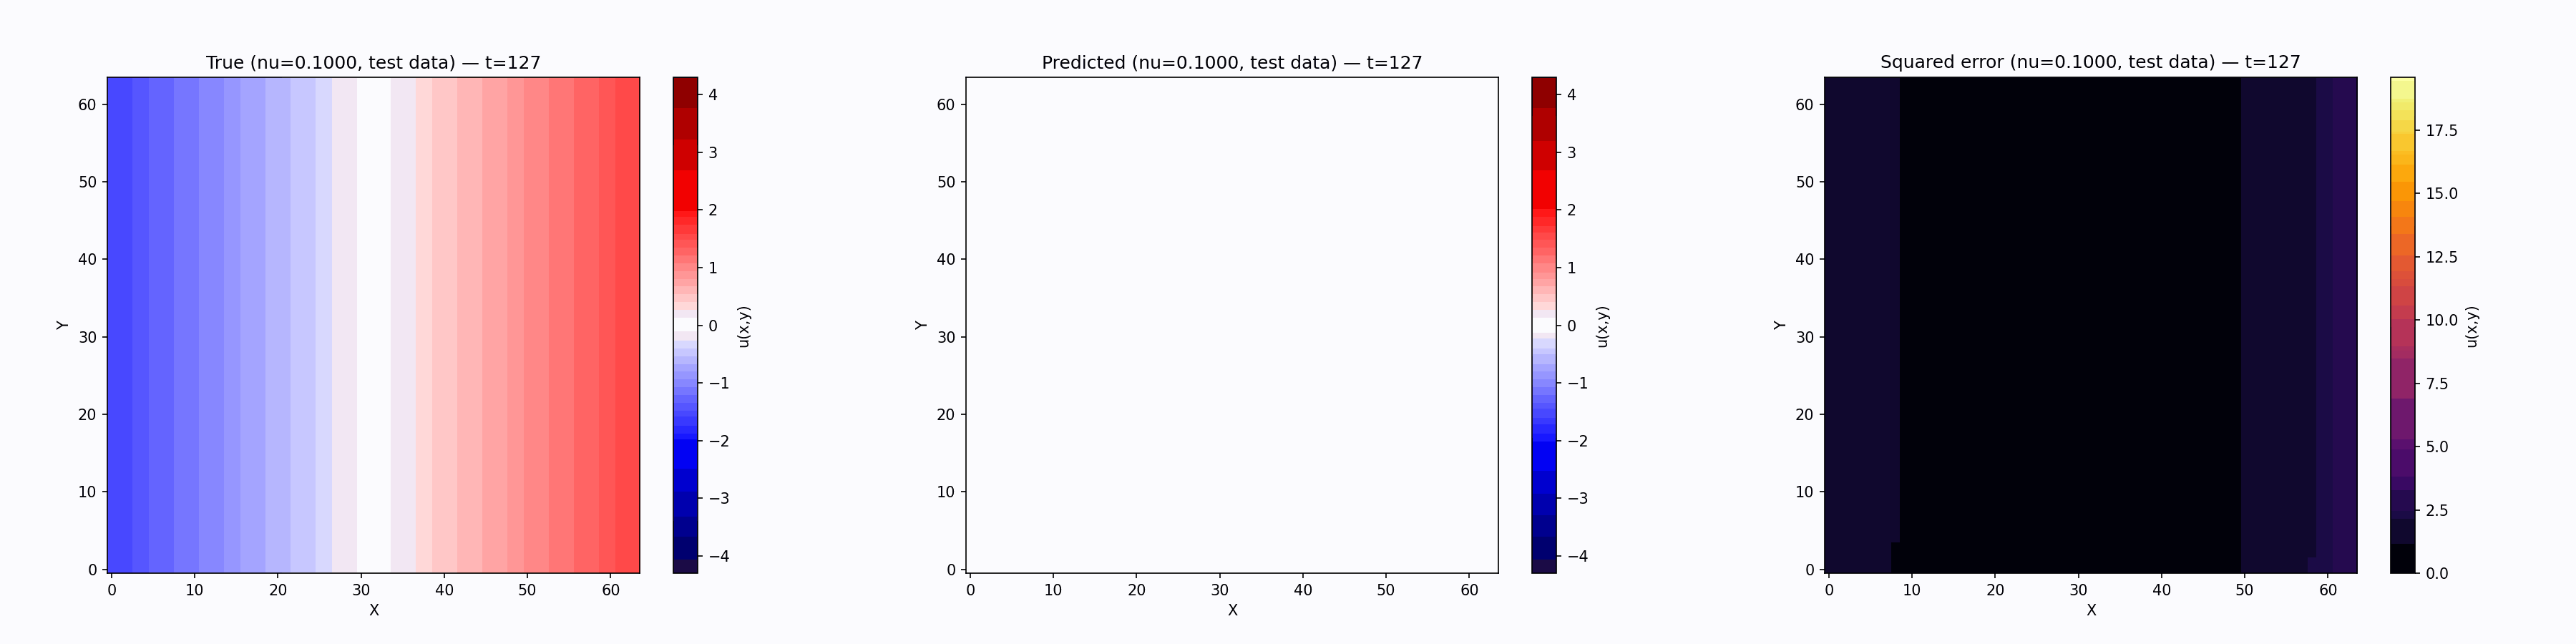
\includegraphics[width=0.80\textwidth]{images/2D_prediction_merged.png}
  \caption{Full rollout comparison for the 2D Burgers model at $\nu=0.1$: ground truth (top) vs.~TCAN prediction (bottom) across 16 time steps. The model captures the global structure but blurs sharp gradients, consistent with the low-frequency bias discussed in Section~\ref{sec:2d_results}.}
  \label{fig:2d-prediction-merged}
\end{figure}

The main factors contributing to this performance gap are:

\begin{enumerate}
    \item \textbf{Higher-dimensional input complexity}: The $(C, H, W)$ field has $2 \times 64 \times 64 = 8192$ values per snapshot, compared to 85--421 values in 1D. The model has fewer effective parameters per spatial degree of freedom.
    \item \textbf{Boundary condition mismatch}: The current implementation uses symmetric (reflect) padding, which does not match the periodic boundary conditions of the Burgers equation, introducing boundary artifacts that propagate inward during autoregressive rollout.
    \item \textbf{Autoregressive error accumulation}: As already observed in 1D, errors compound at each rollout step. The 2D case has more degrees of freedom, so accumulation is faster.
    \item \textbf{Limited training data}: The 2D dataset is substantially smaller than would be needed to cover the viscosity range and initial condition diversity at the same density as the 1D FNO dataset.
\end{enumerate}

%==============================================================================
\section{Planned Improvements and Next Steps}
\label{sec:2d_future_work}
%==============================================================================

Based on the analysis of the preliminary 2D results and the lessons from 1D TCAN, the following improvements are planned:

\paragraph{Boundary condition fix.}
Replace symmetric (reflect) padding with circular padding in all convolutional layers, which is the physically correct choice for a periodic domain.

\paragraph{Progressive rollout training.}
Apply the same progressive rollout curriculum used in 1D to stabilize training in the harder 2D regime. Scheduling exposure to the model's own prediction errors during training~\cite{lippe2023pde} is particularly relevant here.

\paragraph{Larger and more diverse 2D dataset.}
Scale up data generation using a pseudo-spectral solver at multiple resolutions, mirroring the 1D strategy. Active learning~\cite{musekamp2024active} can guide selection of the most informative samples.

\paragraph{Extension to incompressible Navier-Stokes.}
The incompressible Navier-Stokes equations extend the 2D Burgers system with a pressure term and an incompressibility constraint:
\begin{align}
  \frac{\partial \mathbf{u}}{\partial t} + (\mathbf{u} \cdot \nabla)\mathbf{u}
  &= -\nabla p + \nu \nabla^2 \mathbf{u}, \label{eq:ns_momentum} \\[4pt]
  \nabla \cdot \mathbf{u} &= 0. \label{eq:ns_incompressibility}
\end{align}
Handling the pressure field and enforcing the divergence-free condition require additional architectural adaptations (e.g.\ a Hodge-projection correction step), but the TCAN backbone and FiLM viscosity conditioning provide a natural starting point. Successfully extending the NFTM framework to Navier-Stokes would unlock realistic CFD applications at the scale of wing aerodynamics and turbulent channel flows.



\chapter{Conclusion and Perspectives}
\label{chap:conclusion}

This project set out to build a neural architecture capable of learning and advancing the time evolution of physical systems governed by partial differential equations. Starting from the Neural Field Turing Machine (NFTM) framework~\cite{malhotra2025neuralfieldturingmachine}, we investigated a progression of controllers (CNN, Transformer, and TCAN) on the 1D viscous Burgers equation, extended the best-performing model to 2D, and benchmarked it against the Fourier Neural Operator~\cite{li2021fourier}. This chapter summarises our main findings, the limitations we encountered, and the perspectives for future work.

%==============================================================================
\section{Summary of Contributions}
\label{sec:conclusion_summary}
%==============================================================================

\paragraph{Controller comparison.}
We evaluated three controller architectures within the NFTM framework on long-horizon autoregressive rollouts of 1D Burgers dynamics. The CNN controller excels at exploiting local spatial patterns but struggles to capture long-range temporal dependencies, leading to error accumulation over extended rollouts. The Transformer controller handles arbitrary temporal receptive fields, but its cost grows with sequence length and it requires more parameters to match the accuracy of the TCAN. The \textbf{Causal Temporal Convolutional Attention Network (TCAN)} achieves the best results by combining spatial convolutional feature extraction with a causal attention mechanism that also aggregates the full history window. This design, the best of the CNN and Transformer worlds, is the principal model we adopt for all quantitative evaluations.

\paragraph{Viscosity conditioning.}
By passing the viscosity coefficient $\nu$ as an explicit input (via FiLM modulation), a single TCAN model handles dynamics ranging from near-inviscid shock formation ($\nu \approx 0.001$) to strongly diffusive smooth solutions ($\nu \approx 0.5$) without any retraining. This conditioning is essential for generalization: without it, the model trained at one regime fails qualitatively at another.

\paragraph{FNO benchmark and evaluation.}
Switching to the official FNO dataset~\cite{li2021fourier}, generated by the same pseudo-spectral solver used in that paper, allowed us to compare TCAN directly against published baselines (FNO, RBM, FCN, LNO, PCA+NN) at four spatial resolutions ($s \in \{85, 141, 211, 421\}$). At the coarsest resolution ($s=85$), TCAN achieves a relative $L^2$ error of $0.30$, compared to FNO's $0.011$. The results are consistent across resolutions measured by multiple metrics: MSE, SSIM, PSNR, mass conservation, energy monotonicity, and PDE residual.

\paragraph{2D extension.}
We generalised the TCAN architecture to 2D by replacing all 1D spatial operations with their 2D counterparts, retaining FiLM viscosity conditioning, causal temporal attention, and the bounded residual correction. The model trains stably on the 2D Burgers dataset, but the spatial predictions remain qualitatively poor at this stage, motivating the targeted improvements described below.

%==============================================================================
\section{Limitations}
\label{sec:conclusion_limitations}
%==============================================================================

\paragraph{Autoregressive error accumulation.}
The most significant limitation of TCAN relative to FNO is the autoregressive rollout itself. FNO is a \emph{single-step operator} that maps the initial condition directly to $u(\cdot, T)$ in one forward pass. TCAN, by contrast, calls the controller once per time step over $T-1$ steps, allowing small prediction errors to compound exponentially. At finer grids ($s=421$), where more rollout steps are needed per unit time, the relative $L^2$ error reaches $0.94$. Scheduled training on the model's own prediction errors (as in RNO~\cite{lippe2023pderefiner}) is the most direct path to reducing this gap.

\paragraph{Resolution scaling.}
Error grows monotonically with spatial resolution: the same architecture that achieves $0.30$ at $s=85$ reaches $0.94$ at $s=421$. The finer grid requires more time steps in the rollout, and each extra step adds another compounding round of prediction error. Resolution-adaptive training or spectral regularisation could mitigate this effect.

\paragraph{Boundary artifacts.}
The current implementation uses symmetric (reflect) padding in all convolutional layers. For Burgers with periodic boundary conditions, this is physically incorrect: the reflected "mirror image" introduces spurious correlations at the domain edges that propagate inward during the rollout. Replacing reflect padding with circular padding would eliminate this artefact at a negligible implementation cost.

\paragraph{2D model maturity.}
The 2D TCAN is a prototype: it trains without divergence but does not yet produce accurate spatial reconstructions. The dataset is smaller, the boundary padding issue is more severe in 2D, and the optimisation landscape is harder. These are tractable engineering problems rather than fundamental barriers.

%==============================================================================
\section{Perspectives}
\label{sec:conclusion_perspectives}
%==============================================================================

\paragraph{Short-term fixes (1D and 2D).}
The most impactful near-term improvements are: \emph{(i)} replace reflect padding with circular padding; \emph{(ii)} apply progressive rollout training (expose the model to its own errors from the first epoch); and \emph{(iii)} increase the 2D dataset size to match the 1D FNO setup (1000 train / 200 test trajectories per resolution). Together these three changes are expected to close a substantial portion of the FNO gap and lift the 2D model to quantitative accuracy.

\paragraph{Post-processing and physics-based correction.}
PDE-Refiner~\cite{lippe2023pderefiner} can recover sharpness lost at shocks by iterative denoising refinement, applied as a post-processing step on top of TCAN predictions. PhysicsCorrect~\cite{huang2025physicscorrect} offers a training-free projection that reduces PDE residual errors without modifying the architecture. Both approaches are drop-in enhancements compatible with the current TCAN.

\paragraph{Extension to incompressible Navier-Stokes.}
The long-term scientific goal is to simulate 2D incompressible Navier-Stokes:
\begin{align}
  \frac{\partial \mathbf{u}}{\partial t} + (\mathbf{u} \cdot \nabla)\mathbf{u}
  &= -\nabla p + \nu \nabla^2 \mathbf{u}, \\
  \nabla \cdot \mathbf{u} &= 0.
\end{align}
Enforcing the divergence-free constraint $\nabla \cdot \mathbf{u} = 0$ at each rollout step requires an additional Hodge-projection layer (or a learned pressure-correction step) that is absent from the current Burgers architecture. With this addition, the NFTM framework becomes applicable to the full range of incompressible flows, unlocking realistic engineering applications in aerodynamics and heat transfer.

\paragraph{Data efficiency.}
For Navier-Stokes, generating high-fidelity 2D training trajectories is computationally expensive. Active learning~\cite{musekamp2025activelearning}, which intelligently selects the most informative initial conditions and viscosity values for labelling, is a principled way to cover the dynamical parameter space with fewer than 1000 trajectories, and is a natural next step once the 2D Burgers model is stabilised.

%==============================================================================
\section{Key Takeaway}
\label{sec:conclusion_takeaway}
%==============================================================================

This project demonstrates that the NFTM framework with a TCAN controller successfully learns to simulate 1D Burgers dynamics in a data-driven, physics-aware manner. TCAN outperforms the CNN and Transformer baselines on long-horizon rollouts, and viscosity conditioning via FiLM enables a single model to operate across the full range of flow regimes, from sharp shock formation at $\nu \approx 0.001$ to smooth diffusive behaviour at $\nu \approx 0.5$, without retraining.

The performance gap with respect to FNO ($0.30$ vs.\ $0.011$ relative $L^2$ at $s=85$) is not a fundamental architectural limitation but a consequence of the autoregressive formulation: TCAN accumulates small per-step errors over 256 rollout steps, whereas FNO produces a direct one-shot prediction. The identified fixes (circular boundary padding, progressive rollout training, and a larger 2D dataset) are tractable engineering improvements that are expected to close a substantial portion of this gap.

More broadly, this work establishes a solid foundation for generalizable neural PDE solvers. The NFTM framework, with its modular separation of controller and external memory, is well-positioned to scale to 2D incompressible Navier-Stokes once the 1D Burgers bottlenecks are resolved, a promising direction for data-driven simulation of realistic fluid dynamics.


%\appendix

%\include{Appendix1}
%\include{Appendix2}
%\include{Appendix3}
\nocite{*}  % Include all entries in the bibliography
\bibliographystyle{plain}
\bibliography{Thesis}

%\printnomenclature

\cleardoublepage
\begin{vcenterpage}


\noindent{\large\textbf{Abstract:}}
Solving partial differential equations (PDEs) efficiently remains a fundamental challenge in computational physics, with traditional numerical methods often requiring significant computational resources for complex, multi-scale dynamics. This work presents a Neural Field Turing Machine (NFTM) approach for learning PDE solutions, combining external continuous spatial memory with learned read/write operations through a neural controller. We develop and compare three controller architectures—CNN, Transformer, and a Causal Temporal Convolutional Attention Network (TCAN)—as data-driven simulators for the viscous Burgers equation, a canonical nonlinear PDE capturing shock formation and nonlinear advection. TCAN combines spatial convolutions with causal history attention and explicit viscosity conditioning (FiLM), enabling a single model to handle dynamics across the full viscosity range $\nu \in [0, 1]$. Using the official FNO benchmark dataset at four spatial resolutions ($s \in \{85, 141, 211, 421\}$), we evaluate our models against the Fourier Neural Operator (FNO) and related baselines on standard metrics (MSE, SSIM, PSNR) and physics-informed criteria (mass conservation, energy monotonicity, PDE residual). TCAN achieves a relative $L^2$ error of $0.30$ at $s{=}85$, compared to FNO's $0.011$; the gap is attributed to autoregressive error accumulation over 256 rollout steps, as opposed to FNO's single-step operator formulation. We further extend the TCAN architecture to 2D Burgers, demonstrating stable training and identifying boundary padding and dataset scale as the primary factors limiting prediction quality. This framework establishes a foundation for generalizable neural PDE solvers, with planned extensions to incompressible Navier-Stokes equations.
\noindent\rule[2pt]{\textwidth}{0.5pt}
{\large\textbf{Keywords:}}
Neural Field Turing Machines, Physics-Informed Neural Networks, Partial Differential Equations, Burgers Equation, Temporal Convolutional Networks, Attention Mechanisms, Autoregressive Models, Scientific Machine Learning, Computational Fluid Dynamics, Deep Learning for Physics.

\end{vcenterpage}

\end{document}
